\documentclass[twoside]{book}

% Packages required by doxygen
\usepackage{fixltx2e}
\usepackage{calc}
\usepackage{doxygen}
\usepackage[export]{adjustbox} % also loads graphicx
\usepackage{graphicx}
\usepackage[utf8]{inputenc}
\usepackage{makeidx}
\usepackage{multicol}
\usepackage{multirow}
\PassOptionsToPackage{warn}{textcomp}
\usepackage{textcomp}
\usepackage[nointegrals]{wasysym}
\usepackage[table]{xcolor}

% Font selection
\usepackage[T1]{fontenc}
\usepackage[scaled=.90]{helvet}
\usepackage{courier}
\usepackage{amssymb}
\usepackage{sectsty}
\renewcommand{\familydefault}{\sfdefault}
\allsectionsfont{%
  \fontseries{bc}\selectfont%
  \color{darkgray}%
}
\renewcommand{\DoxyLabelFont}{%
  \fontseries{bc}\selectfont%
  \color{darkgray}%
}
\newcommand{\+}{\discretionary{\mbox{\scriptsize$\hookleftarrow$}}{}{}}

% Page & text layout
\usepackage{geometry}
\geometry{%
  a4paper,%
  top=2.5cm,%
  bottom=2.5cm,%
  left=2.5cm,%
  right=2.5cm%
}
\tolerance=750
\hfuzz=15pt
\hbadness=750
\setlength{\emergencystretch}{15pt}
\setlength{\parindent}{0cm}
\setlength{\parskip}{3ex plus 2ex minus 2ex}
\makeatletter
\renewcommand{\paragraph}{%
  \@startsection{paragraph}{4}{0ex}{-1.0ex}{1.0ex}{%
    \normalfont\normalsize\bfseries\SS@parafont%
  }%
}
\renewcommand{\subparagraph}{%
  \@startsection{subparagraph}{5}{0ex}{-1.0ex}{1.0ex}{%
    \normalfont\normalsize\bfseries\SS@subparafont%
  }%
}
\makeatother

% Headers & footers
\usepackage{fancyhdr}
\pagestyle{fancyplain}
\fancyhead[LE]{\fancyplain{}{\bfseries\thepage}}
\fancyhead[CE]{\fancyplain{}{}}
\fancyhead[RE]{\fancyplain{}{\bfseries\leftmark}}
\fancyhead[LO]{\fancyplain{}{\bfseries\rightmark}}
\fancyhead[CO]{\fancyplain{}{}}
\fancyhead[RO]{\fancyplain{}{\bfseries\thepage}}
\fancyfoot[LE]{\fancyplain{}{}}
\fancyfoot[CE]{\fancyplain{}{}}
\fancyfoot[RE]{\fancyplain{}{\bfseries\scriptsize Generated by Doxygen }}
\fancyfoot[LO]{\fancyplain{}{\bfseries\scriptsize Generated by Doxygen }}
\fancyfoot[CO]{\fancyplain{}{}}
\fancyfoot[RO]{\fancyplain{}{}}
\renewcommand{\footrulewidth}{0.4pt}
\renewcommand{\chaptermark}[1]{%
  \markboth{#1}{}%
}
\renewcommand{\sectionmark}[1]{%
  \markright{\thesection\ #1}%
}

% Indices & bibliography
\usepackage{natbib}
\usepackage[titles]{tocloft}
\setcounter{tocdepth}{3}
\setcounter{secnumdepth}{5}
\makeindex

% Hyperlinks (required, but should be loaded last)
\usepackage{ifpdf}
\ifpdf
  \usepackage[pdftex,pagebackref=true]{hyperref}
\else
  \usepackage[ps2pdf,pagebackref=true]{hyperref}
\fi
\hypersetup{%
  colorlinks=true,%
  linkcolor=blue,%
  citecolor=blue,%
  unicode%
}

% Custom commands
\newcommand{\clearemptydoublepage}{%
  \newpage{\pagestyle{empty}\cleardoublepage}%
}

\usepackage{caption}
\captionsetup{labelsep=space,justification=centering,font={bf},singlelinecheck=off,skip=4pt,position=top}

%===== C O N T E N T S =====

\begin{document}

% Titlepage & ToC
\hypersetup{pageanchor=false,
             bookmarksnumbered=true,
             pdfencoding=unicode
            }
\pagenumbering{alph}
\begin{titlepage}
\vspace*{7cm}
\begin{center}%
{\Large My Project }\\
\vspace*{1cm}
{\large Generated by Doxygen 1.8.13}\\
\end{center}
\end{titlepage}
\clearemptydoublepage
\pagenumbering{roman}
\tableofcontents
\clearemptydoublepage
\pagenumbering{arabic}
\hypersetup{pageanchor=true}

%--- Begin generated contents ---
\chapter{Hierarchical Index}
\section{Class Hierarchy}
This inheritance list is sorted roughly, but not completely, alphabetically\+:\begin{DoxyCompactList}
\item \contentsline{section}{util\+:\+:Adresse}{\pageref{classutil_1_1Adresse}}{}
\item \contentsline{section}{elections\+:\+:Circonscription}{\pageref{classelections_1_1Circonscription}}{}
\item \contentsline{section}{util\+:\+:Date}{\pageref{classutil_1_1Date}}{}
\item logic\+\_\+error\begin{DoxyCompactList}
\item \contentsline{section}{Contrat\+Exception}{\pageref{classContratException}}{}
\begin{DoxyCompactList}
\item \contentsline{section}{Assertion\+Exception}{\pageref{classAssertionException}}{}
\item \contentsline{section}{Invariant\+Exception}{\pageref{classInvariantException}}{}
\item \contentsline{section}{Postcondition\+Exception}{\pageref{classPostconditionException}}{}
\item \contentsline{section}{Precondition\+Exception}{\pageref{classPreconditionException}}{}
\end{DoxyCompactList}
\end{DoxyCompactList}
\item \contentsline{section}{elections\+:\+:Personne}{\pageref{classelections_1_1Personne}}{}
\begin{DoxyCompactList}
\item \contentsline{section}{elections\+:\+:Candidat}{\pageref{classelections_1_1Candidat}}{}
\item \contentsline{section}{elections\+:\+:Electeur}{\pageref{classelections_1_1Electeur}}{}
\end{DoxyCompactList}
\end{DoxyCompactList}

\chapter{Class Index}
\section{Class List}
Here are the classes, structs, unions and interfaces with brief descriptions\+:\begin{DoxyCompactList}
\item\contentsline{section}{\hyperlink{classutil_1_1Adresse}{util\+::\+Adresse} \\*Cette classe sert au maintien et à la manipulation des adresses. La classe \hyperlink{classutil_1_1Adresse}{Adresse} permet d\textquotesingle{}implanter des adresses }{\pageref{classutil_1_1Adresse}}{}
\item\contentsline{section}{\hyperlink{classAssertionException}{Assertion\+Exception} \\*Classe pour la gestion des erreurs d\textquotesingle{}assertion }{\pageref{classAssertionException}}{}
\item\contentsline{section}{\hyperlink{classelections_1_1Candidat}{elections\+::\+Candidat} \\*Classe dérivée de la classe \hyperlink{classelections_1_1Personne}{Personne} }{\pageref{classelections_1_1Candidat}}{}
\item\contentsline{section}{\hyperlink{classelections_1_1Circonscription}{elections\+::\+Circonscription} \\*La classe \hyperlink{classelections_1_1Circonscription}{Circonscription} permet de faire la gestion des listes électorales }{\pageref{classelections_1_1Circonscription}}{}
\item\contentsline{section}{\hyperlink{classContratException}{Contrat\+Exception} \\*Classe de base des exceptions de contrat }{\pageref{classContratException}}{}
\item\contentsline{section}{\hyperlink{classutil_1_1Date}{util\+::\+Date} \\*Cette classe sert au maintien et à la manipulation des dates }{\pageref{classutil_1_1Date}}{}
\item\contentsline{section}{\hyperlink{classelections_1_1Electeur}{elections\+::\+Electeur} \\*Classe dérivée de la classe \hyperlink{classelections_1_1Personne}{Personne} }{\pageref{classelections_1_1Electeur}}{}
\item\contentsline{section}{\hyperlink{classInvariantException}{Invariant\+Exception} \\*Classe pour la gestion des erreurs d\textquotesingle{}invariant }{\pageref{classInvariantException}}{}
\item\contentsline{section}{\hyperlink{classelections_1_1Personne}{elections\+::\+Personne} \\*Cette classe sert au maintien et à la manipulation des informations sur une personne. La classe \hyperlink{classelections_1_1Personne}{Personne} permet d\textquotesingle{}implanter des personnes }{\pageref{classelections_1_1Personne}}{}
\item\contentsline{section}{\hyperlink{classPostconditionException}{Postcondition\+Exception} \\*Classe pour la gestion des erreurs de postcondition }{\pageref{classPostconditionException}}{}
\item\contentsline{section}{\hyperlink{classPreconditionException}{Precondition\+Exception} \\*Classe pour la gestion des erreurs de précondition }{\pageref{classPreconditionException}}{}
\end{DoxyCompactList}

\chapter{File Index}
\section{File List}
Here is a list of all documented files with brief descriptions\+:\begin{DoxyCompactList}
\item\contentsline{section}{\hyperlink{Adresse_8cpp}{Adresse.\+cpp} \\*Implantation de la classe Adresse }{\pageref{Adresse_8cpp}}{}
\item\contentsline{section}{\hyperlink{Adresse_8h}{Adresse.\+h} \\*Fichier qui contient l\textquotesingle{}interface de la classe Date qui sert au maintien et à la manipulation des adresses }{\pageref{Adresse_8h}}{}
\item\contentsline{section}{\hyperlink{Candidat_8cpp}{Candidat.\+cpp} \\*Implantation de la classe Candidat }{\pageref{Candidat_8cpp}}{}
\item\contentsline{section}{\hyperlink{Candidat_8h}{Candidat.\+h} \\*Fichier qui contient l\textquotesingle{}interface de la classe Candidat qui sert au maintien et à la manipulation des informations sur un candidat }{\pageref{Candidat_8h}}{}
\item\contentsline{section}{\hyperlink{Circonscription_8cpp}{Circonscription.\+cpp} \\*Implantation de la classe Circonscription }{\pageref{Circonscription_8cpp}}{}
\item\contentsline{section}{\hyperlink{Circonscription_8h}{Circonscription.\+h} \\*Fichier qui contient l\textquotesingle{}interface de la classe Circonscription qui permet de faire la gestion des listes électorales }{\pageref{Circonscription_8h}}{}
\item\contentsline{section}{\hyperlink{ContratException_8cpp}{Contrat\+Exception.\+cpp} \\*Implantation de la classe \hyperlink{classContratException}{Contrat\+Exception} et de ses héritiers }{\pageref{ContratException_8cpp}}{}
\item\contentsline{section}{\hyperlink{ContratException_8h}{Contrat\+Exception.\+h} \\*Fichier contenant la déclaration de la classe \hyperlink{classContratException}{Contrat\+Exception} et de ses héritiers }{\pageref{ContratException_8h}}{}
\item\contentsline{section}{\hyperlink{Date_8cpp}{Date.\+cpp} \\*Implantation de la classe Date révision \+: normes 12-\/2013 balises Doxygen révision des commentaires de spécification d\textquotesingle{}en-\/tête des méthodes }{\pageref{Date_8cpp}}{}
\item\contentsline{section}{\hyperlink{Date_8h}{Date.\+h} \\*Fichier qui contient l\textquotesingle{}interface de la classe Date qui sert au maintien et à la manipulation des dates }{\pageref{Date_8h}}{}
\item\contentsline{section}{\hyperlink{Electeur_8cpp}{Electeur.\+cpp} \\*Implantation de la classe Electeur }{\pageref{Electeur_8cpp}}{}
\item\contentsline{section}{\hyperlink{Electeur_8h}{Electeur.\+h} \\*Fichier qui contient l\textquotesingle{}interface de la classe Electeur qui sert au maintien et à la manipulation des informations sur un electeur }{\pageref{Electeur_8h}}{}
\item\contentsline{section}{\hyperlink{Personne_8cpp}{Personne.\+cpp} \\*Implantation de la classe Personne }{\pageref{Personne_8cpp}}{}
\item\contentsline{section}{\hyperlink{Personne_8h}{Personne.\+h} \\*Fichier qui contient l\textquotesingle{}interface de la classe Personne qui sert au maintien et à la manipulation des informations sur une personne }{\pageref{Personne_8h}}{}
\item\contentsline{section}{\hyperlink{validationFormat_8cpp}{validation\+Format.\+cpp} \\*Fonctions qui permettent de valider un N\+AS et de valider le format d\textquotesingle{}un fichier }{\pageref{validationFormat_8cpp}}{}
\item\contentsline{section}{\hyperlink{validationFormat_8h}{validation\+Format.\+h} \\*Fichier qui contient l\textquotesingle{}interface du fichier de validation d\textquotesingle{}une N\+AS et du format d\textquotesingle{}un fichier }{\pageref{validationFormat_8h}}{}
\end{DoxyCompactList}

\chapter{Class Documentation}
\hypertarget{classutil_1_1Adresse}{}\section{util\+:\+:Adresse Class Reference}
\label{classutil_1_1Adresse}\index{util\+::\+Adresse@{util\+::\+Adresse}}


Cette classe sert au maintien et à la manipulation des adresses. La classe \hyperlink{classutil_1_1Adresse}{Adresse} permet d\textquotesingle{}implanter des adresses.  




{\ttfamily \#include $<$Adresse.\+h$>$}

\subsection*{Public Member Functions}
\begin{DoxyCompactItemize}
\item 
\hyperlink{classutil_1_1Adresse_a2c646a0226925bb32c4db8463ed887d5}{Adresse} (int p\+\_\+numero\+Civic, const std\+::string \&p\+\_\+nom\+Rue, const std\+::string \&p\+\_\+ville, const std\+::string \&p\+\_\+code\+Postal, const std\+::string \&p\+\_\+province)
\begin{DoxyCompactList}\small\item\em Constructeur avec paramètres On construit un objet \hyperlink{classutil_1_1Adresse}{Adresse} à partir de valeurs passées en paramètres. \end{DoxyCompactList}\item 
int \hyperlink{classutil_1_1Adresse_a5b5472020a325014c0296819beba184b}{req\+Numero\+Civic} () const
\begin{DoxyCompactList}\small\item\em retourne le numero civic de l\textquotesingle{}adresse \end{DoxyCompactList}\item 
const std\+::string \& \hyperlink{classutil_1_1Adresse_aa6446c6a166a7ef16700ce5098df4337}{req\+Nom\+Rue} () const
\begin{DoxyCompactList}\small\item\em retourne le nom de la rue de l\textquotesingle{}adresse \end{DoxyCompactList}\item 
const std\+::string \& \hyperlink{classutil_1_1Adresse_a084353601fe763f34dba9ca03af5abe2}{req\+Ville} () const
\begin{DoxyCompactList}\small\item\em retourne le nom de la ville de l\textquotesingle{}adresse \end{DoxyCompactList}\item 
const std\+::string \& \hyperlink{classutil_1_1Adresse_ad4d1a2d82f33ac08b8a647fd479f9edc}{req\+Code\+Postal} () const
\begin{DoxyCompactList}\small\item\em retourne le code postal de l\textquotesingle{}adresse \end{DoxyCompactList}\item 
const std\+::string \& \hyperlink{classutil_1_1Adresse_a9f6048ebc5b0e8bf9a329eb8d9ec2de4}{req\+Province} () const
\begin{DoxyCompactList}\small\item\em retourne le nom de la province de l\textquotesingle{}adresse \end{DoxyCompactList}\item 
void \hyperlink{classutil_1_1Adresse_ab76bad0bb5679f6b091f1bd3b84c5c1b}{asg\+Adresse} (int p\+\_\+numero\+Civic, const std\+::string \&p\+\_\+nom\+Rue, const std\+::string \&p\+\_\+ville, const std\+::string \&p\+\_\+code\+Postal, const std\+::string \&p\+\_\+province)
\begin{DoxyCompactList}\small\item\em Assigne une adresse à l\textquotesingle{}objet courant. \end{DoxyCompactList}\item 
bool \hyperlink{classutil_1_1Adresse_ac622c0ae30e1408c6f5e92e258455c96}{operator==} (const \hyperlink{classutil_1_1Adresse}{Adresse} \&p\+\_\+adresse) const
\begin{DoxyCompactList}\small\item\em surcharge de l\textquotesingle{}opérateur == \end{DoxyCompactList}\item 
std\+::string \hyperlink{classutil_1_1Adresse_ac16f05f371142a65c6f81dea5cce1606}{req\+Adresse\+Formate} () const
\begin{DoxyCompactList}\small\item\em retourne une adresse formatée dans une chaîne de caractères (string) \end{DoxyCompactList}\end{DoxyCompactItemize}


\subsection{Detailed Description}
Cette classe sert au maintien et à la manipulation des adresses. La classe \hyperlink{classutil_1_1Adresse}{Adresse} permet d\textquotesingle{}implanter des adresses. 

\begin{DoxyInvariant}{Invariant}
de la classe\+: le numero\+Civic doit être positif et les nom\+Rue, ville, code\+Postal et province ne doivent pas être vides 
\end{DoxyInvariant}


\subsection{Constructor \& Destructor Documentation}
\mbox{\Hypertarget{classutil_1_1Adresse_a2c646a0226925bb32c4db8463ed887d5}\label{classutil_1_1Adresse_a2c646a0226925bb32c4db8463ed887d5}} 
\index{util\+::\+Adresse@{util\+::\+Adresse}!Adresse@{Adresse}}
\index{Adresse@{Adresse}!util\+::\+Adresse@{util\+::\+Adresse}}
\subsubsection{\texorpdfstring{Adresse()}{Adresse()}}
{\footnotesize\ttfamily util\+::\+Adresse\+::\+Adresse (\begin{DoxyParamCaption}\item[{int}]{p\+\_\+numero\+Civic,  }\item[{const std\+::string \&}]{p\+\_\+nom\+Rue,  }\item[{const std\+::string \&}]{p\+\_\+ville,  }\item[{const std\+::string \&}]{p\+\_\+code\+Postal,  }\item[{const std\+::string \&}]{p\+\_\+province }\end{DoxyParamCaption})}



Constructeur avec paramètres On construit un objet \hyperlink{classutil_1_1Adresse}{Adresse} à partir de valeurs passées en paramètres. 


\begin{DoxyParams}[1]{Parameters}
\mbox{\tt in}  & {\em p\+\_\+numero\+Civic} & est un entier int qui représente le numero civic de l\textquotesingle{}adresse \\
\hline
\mbox{\tt in}  & {\em p\+\_\+nom\+Rue} & est une string qui représente le nom de la rue de l\textquotesingle{}adresse \\
\hline
\mbox{\tt in}  & {\em p\+\_\+ville} & est une string qui représente le nom de la ville de l\textquotesingle{}adresse \\
\hline
\mbox{\tt in}  & {\em p\+\_\+code\+Postal} & est une string qui représente le code postal de l\textquotesingle{}adresse \\
\hline
\mbox{\tt in}  & {\em p\+\_\+province} & est une string qui représente le nom de la province de l\textquotesingle{}adresse \\
\hline
\end{DoxyParams}
\begin{DoxyPrecond}{Precondition}
p\+\_\+numero\+Civic doit être un nombre positif. 

p\+\_\+nom\+Rue doit être non vide. 

p\+\_\+ville doit être non vide. 

p\+\_\+code\+Postal doit être non vide. 

p\+\_\+province doit être non vide. 
\end{DoxyPrecond}
\begin{DoxyPostcond}{Postcondition}
m\+\_\+numero\+Civic prend la valeur du paramètre reçu en entrée. 

m\+\_\+nom\+Rue prend la valeur du paramètre reçu en entrée. 

m\+\_\+ville prend la valeur du paramètre reçu en entrée. 

m\+\_\+code\+Postal prend la valeur du paramètre reçu en entrée. 

m\+\_\+province prend la valeur du paramètre reçu en entrée. 
\end{DoxyPostcond}


\subsection{Member Function Documentation}
\mbox{\Hypertarget{classutil_1_1Adresse_ab76bad0bb5679f6b091f1bd3b84c5c1b}\label{classutil_1_1Adresse_ab76bad0bb5679f6b091f1bd3b84c5c1b}} 
\index{util\+::\+Adresse@{util\+::\+Adresse}!asg\+Adresse@{asg\+Adresse}}
\index{asg\+Adresse@{asg\+Adresse}!util\+::\+Adresse@{util\+::\+Adresse}}
\subsubsection{\texorpdfstring{asg\+Adresse()}{asgAdresse()}}
{\footnotesize\ttfamily void util\+::\+Adresse\+::asg\+Adresse (\begin{DoxyParamCaption}\item[{int}]{p\+\_\+numero\+Civic,  }\item[{const std\+::string \&}]{p\+\_\+nom\+Rue,  }\item[{const std\+::string \&}]{p\+\_\+ville,  }\item[{const std\+::string \&}]{p\+\_\+code\+Postal,  }\item[{const std\+::string \&}]{p\+\_\+province }\end{DoxyParamCaption})}



Assigne une adresse à l\textquotesingle{}objet courant. 


\begin{DoxyParams}[1]{Parameters}
\mbox{\tt in}  & {\em p\+\_\+numero\+Civic} & est un entier int qui représente le numero civic de l\textquotesingle{}adresse \\
\hline
\mbox{\tt in}  & {\em p\+\_\+nom\+Rue} & est une string qui représente le nom de la rue de l\textquotesingle{}adresse \\
\hline
\mbox{\tt in}  & {\em p\+\_\+ville} & est une string qui représente le nom de la ville de l\textquotesingle{}adresse \\
\hline
\mbox{\tt in}  & {\em p\+\_\+code\+Postal} & est une string qui représente le code postal de l\textquotesingle{}adresse \\
\hline
\mbox{\tt in}  & {\em p\+\_\+province} & est une string qui représente le nom de la province de l\textquotesingle{}adresse \\
\hline
\end{DoxyParams}
\begin{DoxyPrecond}{Precondition}
p\+\_\+numero\+Civic doit être un nombre positif. 

p\+\_\+nom\+Rue doit être un nombre positif. 

p\+\_\+ville doit être un nombre positif. 

p\+\_\+code\+Postal doit être un nombre positif. 

p\+\_\+province doit être un nombre positif. 
\end{DoxyPrecond}
\begin{DoxyPostcond}{Postcondition}
m\+\_\+numero\+Civic prend la valeur du paramètre reçu en entrée. 

m\+\_\+nom\+Rue prend la valeur du paramètre reçu en entrée. 

m\+\_\+ville prend la valeur du paramètre reçu en entrée. 

m\+\_\+code\+Postal prend la valeur du paramètre reçu en entrée. 

m\+\_\+province prend la valeur du paramètre reçu en entrée. 
\end{DoxyPostcond}
\mbox{\Hypertarget{classutil_1_1Adresse_ac622c0ae30e1408c6f5e92e258455c96}\label{classutil_1_1Adresse_ac622c0ae30e1408c6f5e92e258455c96}} 
\index{util\+::\+Adresse@{util\+::\+Adresse}!operator==@{operator==}}
\index{operator==@{operator==}!util\+::\+Adresse@{util\+::\+Adresse}}
\subsubsection{\texorpdfstring{operator==()}{operator==()}}
{\footnotesize\ttfamily bool util\+::\+Adresse\+::operator== (\begin{DoxyParamCaption}\item[{const \hyperlink{classutil_1_1Adresse}{Adresse} \&}]{p\+\_\+adresse }\end{DoxyParamCaption}) const}



surcharge de l\textquotesingle{}opérateur == 


\begin{DoxyParams}[1]{Parameters}
\mbox{\tt in}  & {\em p\+\_\+adresse} & qui est une adresse valide \\
\hline
\end{DoxyParams}
\begin{DoxyReturn}{Returns}
un booléen indiquant si deux attributs d\textquotesingle{}une adresse sont égales ou pas 
\end{DoxyReturn}
\mbox{\Hypertarget{classutil_1_1Adresse_ac16f05f371142a65c6f81dea5cce1606}\label{classutil_1_1Adresse_ac16f05f371142a65c6f81dea5cce1606}} 
\index{util\+::\+Adresse@{util\+::\+Adresse}!req\+Adresse\+Formate@{req\+Adresse\+Formate}}
\index{req\+Adresse\+Formate@{req\+Adresse\+Formate}!util\+::\+Adresse@{util\+::\+Adresse}}
\subsubsection{\texorpdfstring{req\+Adresse\+Formate()}{reqAdresseFormate()}}
{\footnotesize\ttfamily string util\+::\+Adresse\+::req\+Adresse\+Formate (\begin{DoxyParamCaption}{ }\end{DoxyParamCaption}) const}



retourne une adresse formatée dans une chaîne de caractères (string) 

\begin{DoxyReturn}{Returns}
une adresse formatée dans une chaîne de caractères 
\end{DoxyReturn}
\mbox{\Hypertarget{classutil_1_1Adresse_ad4d1a2d82f33ac08b8a647fd479f9edc}\label{classutil_1_1Adresse_ad4d1a2d82f33ac08b8a647fd479f9edc}} 
\index{util\+::\+Adresse@{util\+::\+Adresse}!req\+Code\+Postal@{req\+Code\+Postal}}
\index{req\+Code\+Postal@{req\+Code\+Postal}!util\+::\+Adresse@{util\+::\+Adresse}}
\subsubsection{\texorpdfstring{req\+Code\+Postal()}{reqCodePostal()}}
{\footnotesize\ttfamily const string \& util\+::\+Adresse\+::req\+Code\+Postal (\begin{DoxyParamCaption}{ }\end{DoxyParamCaption}) const}



retourne le code postal de l\textquotesingle{}adresse 

\begin{DoxyReturn}{Returns}
une string qui représente le code postal de l\textquotesingle{}adresse 
\end{DoxyReturn}
\mbox{\Hypertarget{classutil_1_1Adresse_aa6446c6a166a7ef16700ce5098df4337}\label{classutil_1_1Adresse_aa6446c6a166a7ef16700ce5098df4337}} 
\index{util\+::\+Adresse@{util\+::\+Adresse}!req\+Nom\+Rue@{req\+Nom\+Rue}}
\index{req\+Nom\+Rue@{req\+Nom\+Rue}!util\+::\+Adresse@{util\+::\+Adresse}}
\subsubsection{\texorpdfstring{req\+Nom\+Rue()}{reqNomRue()}}
{\footnotesize\ttfamily const string \& util\+::\+Adresse\+::req\+Nom\+Rue (\begin{DoxyParamCaption}{ }\end{DoxyParamCaption}) const}



retourne le nom de la rue de l\textquotesingle{}adresse 

\begin{DoxyReturn}{Returns}
une string qui représente le nom de la rue de l\textquotesingle{}adresse 
\end{DoxyReturn}
\mbox{\Hypertarget{classutil_1_1Adresse_a5b5472020a325014c0296819beba184b}\label{classutil_1_1Adresse_a5b5472020a325014c0296819beba184b}} 
\index{util\+::\+Adresse@{util\+::\+Adresse}!req\+Numero\+Civic@{req\+Numero\+Civic}}
\index{req\+Numero\+Civic@{req\+Numero\+Civic}!util\+::\+Adresse@{util\+::\+Adresse}}
\subsubsection{\texorpdfstring{req\+Numero\+Civic()}{reqNumeroCivic()}}
{\footnotesize\ttfamily int util\+::\+Adresse\+::req\+Numero\+Civic (\begin{DoxyParamCaption}{ }\end{DoxyParamCaption}) const}



retourne le numero civic de l\textquotesingle{}adresse 

\begin{DoxyReturn}{Returns}
un entier int qui représente le numero civic de l\textquotesingle{}adresse 
\end{DoxyReturn}
\mbox{\Hypertarget{classutil_1_1Adresse_a9f6048ebc5b0e8bf9a329eb8d9ec2de4}\label{classutil_1_1Adresse_a9f6048ebc5b0e8bf9a329eb8d9ec2de4}} 
\index{util\+::\+Adresse@{util\+::\+Adresse}!req\+Province@{req\+Province}}
\index{req\+Province@{req\+Province}!util\+::\+Adresse@{util\+::\+Adresse}}
\subsubsection{\texorpdfstring{req\+Province()}{reqProvince()}}
{\footnotesize\ttfamily const string \& util\+::\+Adresse\+::req\+Province (\begin{DoxyParamCaption}{ }\end{DoxyParamCaption}) const}



retourne le nom de la province de l\textquotesingle{}adresse 

\begin{DoxyReturn}{Returns}
une string qui représente le nom de la province de l\textquotesingle{}adresse 
\end{DoxyReturn}
\mbox{\Hypertarget{classutil_1_1Adresse_a084353601fe763f34dba9ca03af5abe2}\label{classutil_1_1Adresse_a084353601fe763f34dba9ca03af5abe2}} 
\index{util\+::\+Adresse@{util\+::\+Adresse}!req\+Ville@{req\+Ville}}
\index{req\+Ville@{req\+Ville}!util\+::\+Adresse@{util\+::\+Adresse}}
\subsubsection{\texorpdfstring{req\+Ville()}{reqVille()}}
{\footnotesize\ttfamily const string \& util\+::\+Adresse\+::req\+Ville (\begin{DoxyParamCaption}{ }\end{DoxyParamCaption}) const}



retourne le nom de la ville de l\textquotesingle{}adresse 

\begin{DoxyReturn}{Returns}
une string qui représente le nom de la ville de l\textquotesingle{}adresse 
\end{DoxyReturn}


The documentation for this class was generated from the following files\+:\begin{DoxyCompactItemize}
\item 
\hyperlink{Adresse_8h}{Adresse.\+h}\item 
\hyperlink{Adresse_8cpp}{Adresse.\+cpp}\end{DoxyCompactItemize}

\hypertarget{classAssertionException}{}\section{Assertion\+Exception Class Reference}
\label{classAssertionException}\index{Assertion\+Exception@{Assertion\+Exception}}


Classe pour la gestion des erreurs d\textquotesingle{}assertion.  




{\ttfamily \#include $<$Contrat\+Exception.\+h$>$}



Inheritance diagram for Assertion\+Exception\+:\nopagebreak
\begin{figure}[H]
\begin{center}
\leavevmode
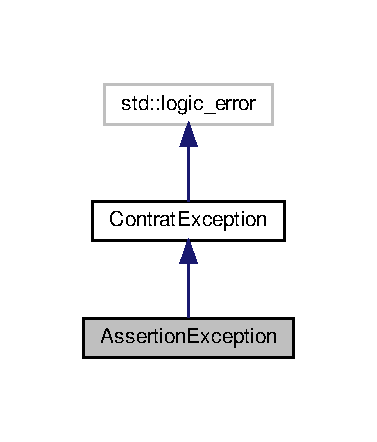
\includegraphics[width=181pt]{classAssertionException__inherit__graph}
\end{center}
\end{figure}


Collaboration diagram for Assertion\+Exception\+:\nopagebreak
\begin{figure}[H]
\begin{center}
\leavevmode
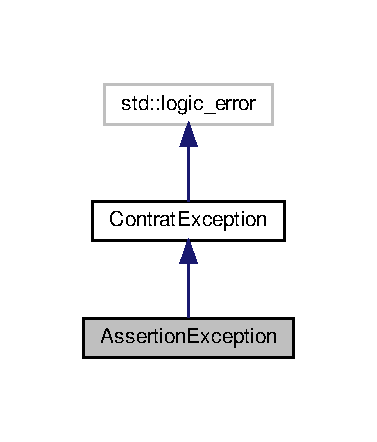
\includegraphics[width=181pt]{classAssertionException__coll__graph}
\end{center}
\end{figure}
\subsection*{Public Member Functions}
\begin{DoxyCompactItemize}
\item 
\hyperlink{classAssertionException_a93268f249b033bf4596901e50874fde6}{Assertion\+Exception} (std\+::string, unsigned int, std\+::string)
\begin{DoxyCompactList}\small\item\em Constructeur de la classe \hyperlink{classAssertionException}{Assertion\+Exception} ~\newline
 Le constructeur public \hyperlink{classAssertionException}{Assertion\+Exception}(...)initialise sa classe de base \hyperlink{classContratException}{Contrat\+Exception}. On n\textquotesingle{}a pas d\textquotesingle{}attribut local. Cette classe est intéressante pour son T\+Y\+PE lors du traitement des exceptions. \end{DoxyCompactList}\end{DoxyCompactItemize}


\subsection{Detailed Description}
Classe pour la gestion des erreurs d\textquotesingle{}assertion. 

\subsection{Constructor \& Destructor Documentation}
\mbox{\Hypertarget{classAssertionException_a93268f249b033bf4596901e50874fde6}\label{classAssertionException_a93268f249b033bf4596901e50874fde6}} 
\index{Assertion\+Exception@{Assertion\+Exception}!Assertion\+Exception@{Assertion\+Exception}}
\index{Assertion\+Exception@{Assertion\+Exception}!Assertion\+Exception@{Assertion\+Exception}}
\subsubsection{\texorpdfstring{Assertion\+Exception()}{AssertionException()}}
{\footnotesize\ttfamily Assertion\+Exception\+::\+Assertion\+Exception (\begin{DoxyParamCaption}\item[{std\+::string}]{p\+\_\+fichP,  }\item[{unsigned int}]{p\+\_\+prm\+Ligne,  }\item[{std\+::string}]{p\+\_\+exprP }\end{DoxyParamCaption})}



Constructeur de la classe \hyperlink{classAssertionException}{Assertion\+Exception} ~\newline
 Le constructeur public \hyperlink{classAssertionException}{Assertion\+Exception}(...)initialise sa classe de base \hyperlink{classContratException}{Contrat\+Exception}. On n\textquotesingle{}a pas d\textquotesingle{}attribut local. Cette classe est intéressante pour son T\+Y\+PE lors du traitement des exceptions. 


\begin{DoxyParams}{Parameters}
{\em p\+\_\+fichP} & chaîne de caractères représentant le fichier source dans lequel a eu lieu l\textquotesingle{}erreur \\
\hline
{\em p\+\_\+prm\+Ligne} & un entier représentant la ligne où a eu lieu l\textquotesingle{}erreur \\
\hline
{\em p\+\_\+exprP} & Test logique qui a échoué \\
\hline
\end{DoxyParams}


The documentation for this class was generated from the following files\+:\begin{DoxyCompactItemize}
\item 
\hyperlink{ContratException_8h}{Contrat\+Exception.\+h}\item 
\hyperlink{ContratException_8cpp}{Contrat\+Exception.\+cpp}\end{DoxyCompactItemize}

\hypertarget{classelections_1_1Candidat}{}\section{elections\+:\+:Candidat Class Reference}
\label{classelections_1_1Candidat}\index{elections\+::\+Candidat@{elections\+::\+Candidat}}


Classe dérivée de la classe \hyperlink{classelections_1_1Personne}{Personne}.  




{\ttfamily \#include $<$Candidat.\+h$>$}



Inheritance diagram for elections\+:\+:Candidat\+:\nopagebreak
\begin{figure}[H]
\begin{center}
\leavevmode
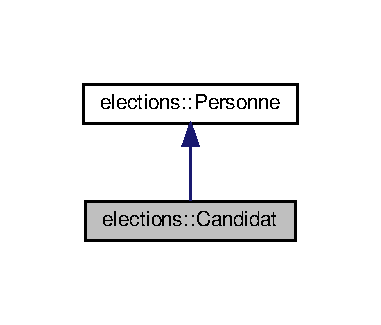
\includegraphics[width=183pt]{classelections_1_1Candidat__inherit__graph}
\end{center}
\end{figure}


Collaboration diagram for elections\+:\+:Candidat\+:\nopagebreak
\begin{figure}[H]
\begin{center}
\leavevmode
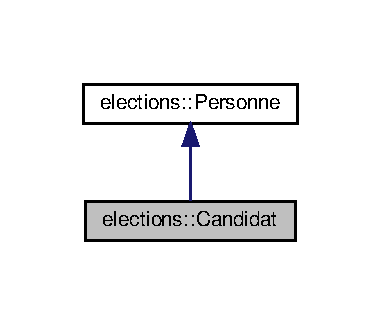
\includegraphics[width=183pt]{classelections_1_1Candidat__coll__graph}
\end{center}
\end{figure}
\subsection*{Public Member Functions}
\begin{DoxyCompactItemize}
\item 
\hyperlink{classelections_1_1Candidat_a543dcf32971b2fc7c8fe984ea007c83a}{Candidat} (const string \&p\+\_\+nas, const string \&p\+\_\+prenom, const string \&p\+\_\+nom, const \hyperlink{classutil_1_1Date}{util\+::\+Date} \&p\+\_\+date\+Naissance, const \hyperlink{classutil_1_1Adresse}{util\+::\+Adresse} \&p\+\_\+adresse, int p\+\_\+parti\+Politique)
\begin{DoxyCompactList}\small\item\em Constructeur avec paramètre Création d\textquotesingle{}un objet \hyperlink{classelections_1_1Candidat}{Candidat} à partir de valeurs passées en paramètres. \end{DoxyCompactList}\item 
virtual \hyperlink{classelections_1_1Personne}{Personne} $\ast$ \hyperlink{classelections_1_1Candidat_ac93fed3409eb4617620d70a1d031ae89}{clone} () const
\begin{DoxyCompactList}\small\item\em \hyperlink{classelections_1_1Candidat_ac93fed3409eb4617620d70a1d031ae89}{clone()} permet de faire une copie allouée sur le monceau de l\textquotesingle{}objet courant \end{DoxyCompactList}\item 
int \hyperlink{classelections_1_1Candidat_a150b2e680fbea708f222e5e8bfd823e4}{req\+Parti\+Politique} () const
\begin{DoxyCompactList}\small\item\em Accesseur sur le parti politique du candidat. \end{DoxyCompactList}\item 
virtual std\+::string \hyperlink{classelections_1_1Candidat_a4b614df7326d8aacdec158b77a6ec406}{req\+Personne\+Formate} () const
\begin{DoxyCompactList}\small\item\em Affiche les informations du candidat sous forme d\textquotesingle{}une chaîne de caractère formatée. \end{DoxyCompactList}\end{DoxyCompactItemize}


\subsection{Detailed Description}
Classe dérivée de la classe \hyperlink{classelections_1_1Personne}{Personne}. 

\begin{DoxyInvariant}{Invariant}
de la classe\+: le parti politique doit etre un chiffre de 0 a 4 
\end{DoxyInvariant}


\subsection{Constructor \& Destructor Documentation}
\mbox{\Hypertarget{classelections_1_1Candidat_a543dcf32971b2fc7c8fe984ea007c83a}\label{classelections_1_1Candidat_a543dcf32971b2fc7c8fe984ea007c83a}} 
\index{elections\+::\+Candidat@{elections\+::\+Candidat}!Candidat@{Candidat}}
\index{Candidat@{Candidat}!elections\+::\+Candidat@{elections\+::\+Candidat}}
\subsubsection{\texorpdfstring{Candidat()}{Candidat()}}
{\footnotesize\ttfamily elections\+::\+Candidat\+::\+Candidat (\begin{DoxyParamCaption}\item[{const string \&}]{p\+\_\+nas,  }\item[{const string \&}]{p\+\_\+prenom,  }\item[{const string \&}]{p\+\_\+nom,  }\item[{const \hyperlink{classutil_1_1Date}{util\+::\+Date} \&}]{p\+\_\+date\+Naissance,  }\item[{const \hyperlink{classutil_1_1Adresse}{util\+::\+Adresse} \&}]{p\+\_\+adresse,  }\item[{int}]{p\+\_\+parti\+Politique }\end{DoxyParamCaption})}



Constructeur avec paramètre Création d\textquotesingle{}un objet \hyperlink{classelections_1_1Candidat}{Candidat} à partir de valeurs passées en paramètres. 


\begin{DoxyParams}[1]{Parameters}
\mbox{\tt in}  & {\em p\+\_\+nas} & nas du candidat \\
\hline
\mbox{\tt in}  & {\em p\+\_\+prenom} & prenom du candidat \\
\hline
\mbox{\tt in}  & {\em p\+\_\+nom} & nom du candidat \\
\hline
\mbox{\tt in}  & {\em p\+\_\+date\+Naissance} & date de naissance du candidat \\
\hline
\mbox{\tt in}  & {\em p\+\_\+adresse} & adresse du candidat \\
\hline
\mbox{\tt in}  & {\em p\+\_\+parti\+Politique} & parti politique pour lequel le candidat se presente \\
\hline
\end{DoxyParams}
\begin{DoxyPrecond}{Precondition}
parti politique valide 
\end{DoxyPrecond}
\begin{DoxyPostcond}{Postcondition}
m\+\_\+parti\+Politique prend la valeur de p\+\_\+parti\+Politique 
\end{DoxyPostcond}


\subsection{Member Function Documentation}
\mbox{\Hypertarget{classelections_1_1Candidat_ac93fed3409eb4617620d70a1d031ae89}\label{classelections_1_1Candidat_ac93fed3409eb4617620d70a1d031ae89}} 
\index{elections\+::\+Candidat@{elections\+::\+Candidat}!clone@{clone}}
\index{clone@{clone}!elections\+::\+Candidat@{elections\+::\+Candidat}}
\subsubsection{\texorpdfstring{clone()}{clone()}}
{\footnotesize\ttfamily \hyperlink{classelections_1_1Personne}{Personne} $\ast$ elections\+::\+Candidat\+::clone (\begin{DoxyParamCaption}{ }\end{DoxyParamCaption}) const\hspace{0.3cm}{\ttfamily [virtual]}}



\hyperlink{classelections_1_1Candidat_ac93fed3409eb4617620d70a1d031ae89}{clone()} permet de faire une copie allouée sur le monceau de l\textquotesingle{}objet courant 

\begin{DoxyReturn}{Returns}
pointeur de candidat 
\end{DoxyReturn}


Implements \hyperlink{classelections_1_1Personne}{elections\+::\+Personne}.

\mbox{\Hypertarget{classelections_1_1Candidat_a150b2e680fbea708f222e5e8bfd823e4}\label{classelections_1_1Candidat_a150b2e680fbea708f222e5e8bfd823e4}} 
\index{elections\+::\+Candidat@{elections\+::\+Candidat}!req\+Parti\+Politique@{req\+Parti\+Politique}}
\index{req\+Parti\+Politique@{req\+Parti\+Politique}!elections\+::\+Candidat@{elections\+::\+Candidat}}
\subsubsection{\texorpdfstring{req\+Parti\+Politique()}{reqPartiPolitique()}}
{\footnotesize\ttfamily int elections\+::\+Candidat\+::req\+Parti\+Politique (\begin{DoxyParamCaption}{ }\end{DoxyParamCaption}) const}



Accesseur sur le parti politique du candidat. 

\begin{DoxyReturn}{Returns}
le parti politique du candidat 
\end{DoxyReturn}
\mbox{\Hypertarget{classelections_1_1Candidat_a4b614df7326d8aacdec158b77a6ec406}\label{classelections_1_1Candidat_a4b614df7326d8aacdec158b77a6ec406}} 
\index{elections\+::\+Candidat@{elections\+::\+Candidat}!req\+Personne\+Formate@{req\+Personne\+Formate}}
\index{req\+Personne\+Formate@{req\+Personne\+Formate}!elections\+::\+Candidat@{elections\+::\+Candidat}}
\subsubsection{\texorpdfstring{req\+Personne\+Formate()}{reqPersonneFormate()}}
{\footnotesize\ttfamily string elections\+::\+Candidat\+::req\+Personne\+Formate (\begin{DoxyParamCaption}{ }\end{DoxyParamCaption}) const\hspace{0.3cm}{\ttfamily [virtual]}}



Affiche les informations du candidat sous forme d\textquotesingle{}une chaîne de caractère formatée. 

\begin{DoxyReturn}{Returns}
les informations sur un candidat 
\end{DoxyReturn}


Implements \hyperlink{classelections_1_1Personne_aac1232e61b7cb9743bafba9280041d35}{elections\+::\+Personne}.



The documentation for this class was generated from the following files\+:\begin{DoxyCompactItemize}
\item 
\hyperlink{Candidat_8h}{Candidat.\+h}\item 
\hyperlink{Candidat_8cpp}{Candidat.\+cpp}\end{DoxyCompactItemize}

\hypertarget{classelections_1_1Circonscription}{}\section{elections\+:\+:Circonscription Class Reference}
\label{classelections_1_1Circonscription}\index{elections\+::\+Circonscription@{elections\+::\+Circonscription}}


La classe \hyperlink{classelections_1_1Circonscription}{Circonscription} permet de faire la gestion des listes électorales.  




{\ttfamily \#include $<$Circonscription.\+h$>$}

\subsection*{Public Member Functions}
\begin{DoxyCompactItemize}
\item 
\hyperlink{classelections_1_1Circonscription_a73b7ff6d629d356fc9a38337848d5e00}{Circonscription} (const string \&p\+\_\+nom\+Circonscription, const \hyperlink{classelections_1_1Candidat}{elections\+::\+Candidat} \&p\+\_\+depute\+Elu)
\begin{DoxyCompactList}\small\item\em Constructeur avec paramètre Création d\textquotesingle{}un objet \hyperlink{classelections_1_1Circonscription}{Circonscription} à partir de valeurs passées en paramètres. \end{DoxyCompactList}\item 
\mbox{\Hypertarget{classelections_1_1Circonscription_abc80c8b4c096dfc36a55cc0e7b8d3a8c}\label{classelections_1_1Circonscription_abc80c8b4c096dfc36a55cc0e7b8d3a8c}} 
\hyperlink{classelections_1_1Circonscription_abc80c8b4c096dfc36a55cc0e7b8d3a8c}{$\sim$\+Circonscription} ()
\begin{DoxyCompactList}\small\item\em Destructeur responsable de désallouer toutes les Personnes de la liste dans le vecteur. \end{DoxyCompactList}\item 
const std\+::string \& \hyperlink{classelections_1_1Circonscription_adbacabf731fe2afccc919b8bd8c4eae8}{req\+Nom\+Circonscription} () const
\begin{DoxyCompactList}\small\item\em retourne le nom de la circonscription \end{DoxyCompactList}\item 
const \hyperlink{classelections_1_1Candidat}{elections\+::\+Candidat} \& \hyperlink{classelections_1_1Circonscription_a162a8ccd10bbfe3297489e19e924f3d1}{req\+Depute\+Elu} () const
\begin{DoxyCompactList}\small\item\em retourne le candidat sortant d\textquotesingle{}une circonscription \end{DoxyCompactList}\item 
void \hyperlink{classelections_1_1Circonscription_a808d1495bfb8dda4bb75114d3387d35b}{inscrire} (const \hyperlink{classelections_1_1Personne}{Personne} \&p\+\_\+nouvel\+Inscrit)
\begin{DoxyCompactList}\small\item\em Methode qui permet d’inscrire une personne sur la liste électorale de la circonscription. \end{DoxyCompactList}\item 
\hyperlink{classelections_1_1Circonscription_ab97d93c0108451f646ec8101caa39999}{Circonscription} (const \hyperlink{classelections_1_1Circonscription}{Circonscription} \&p\+\_\+circonscription)
\begin{DoxyCompactList}\small\item\em Constructeur copie Création d\textquotesingle{}un objet \hyperlink{classelections_1_1Circonscription}{Circonscription} copie a partie d’un autre objet \hyperlink{classelections_1_1Circonscription}{Circonscription}. \end{DoxyCompactList}\item 
const \hyperlink{classelections_1_1Circonscription}{Circonscription} \& \hyperlink{classelections_1_1Circonscription_ab61ae982ba5f251ee1ac20bd660498b1}{operator=} (const \hyperlink{classelections_1_1Circonscription}{Circonscription} \&p\+\_\+circonscription)
\begin{DoxyCompactList}\small\item\em surcharge de l\textquotesingle{}opérateur = \end{DoxyCompactList}\item 
std\+::string \hyperlink{classelections_1_1Circonscription_aeea7de1ad15f781187aec0f0e01a14f4}{req\+Circonscription\+Formate} () const
\begin{DoxyCompactList}\small\item\em Affiche les informations de la circonscription sous forme d\textquotesingle{}une chaîne de caractère formatée. \end{DoxyCompactList}\end{DoxyCompactItemize}


\subsection{Detailed Description}
La classe \hyperlink{classelections_1_1Circonscription}{Circonscription} permet de faire la gestion des listes électorales. 

\begin{DoxyInvariant}{Invariant}
de la classe\+: le nom de la circonscription ne doit pas etre vide 
\end{DoxyInvariant}


\subsection{Constructor \& Destructor Documentation}
\mbox{\Hypertarget{classelections_1_1Circonscription_a73b7ff6d629d356fc9a38337848d5e00}\label{classelections_1_1Circonscription_a73b7ff6d629d356fc9a38337848d5e00}} 
\index{elections\+::\+Circonscription@{elections\+::\+Circonscription}!Circonscription@{Circonscription}}
\index{Circonscription@{Circonscription}!elections\+::\+Circonscription@{elections\+::\+Circonscription}}
\subsubsection{\texorpdfstring{Circonscription()}{Circonscription()}\hspace{0.1cm}{\footnotesize\ttfamily [1/2]}}
{\footnotesize\ttfamily elections\+::\+Circonscription\+::\+Circonscription (\begin{DoxyParamCaption}\item[{const string \&}]{p\+\_\+nom\+Circonscription,  }\item[{const \hyperlink{classelections_1_1Candidat}{elections\+::\+Candidat} \&}]{p\+\_\+depute\+Elu }\end{DoxyParamCaption})}



Constructeur avec paramètre Création d\textquotesingle{}un objet \hyperlink{classelections_1_1Circonscription}{Circonscription} à partir de valeurs passées en paramètres. 


\begin{DoxyParams}[1]{Parameters}
\mbox{\tt in}  & {\em p\+\_\+nom\+Circonscription} & nom de la circonscription \\
\hline
\mbox{\tt in}  & {\em p\+\_\+depute\+Elu} & depute elu sortant \\
\hline
\end{DoxyParams}
\mbox{\Hypertarget{classelections_1_1Circonscription_ab97d93c0108451f646ec8101caa39999}\label{classelections_1_1Circonscription_ab97d93c0108451f646ec8101caa39999}} 
\index{elections\+::\+Circonscription@{elections\+::\+Circonscription}!Circonscription@{Circonscription}}
\index{Circonscription@{Circonscription}!elections\+::\+Circonscription@{elections\+::\+Circonscription}}
\subsubsection{\texorpdfstring{Circonscription()}{Circonscription()}\hspace{0.1cm}{\footnotesize\ttfamily [2/2]}}
{\footnotesize\ttfamily elections\+::\+Circonscription\+::\+Circonscription (\begin{DoxyParamCaption}\item[{const \hyperlink{classelections_1_1Circonscription}{Circonscription} \&}]{p\+\_\+circonscription }\end{DoxyParamCaption})}



Constructeur copie Création d\textquotesingle{}un objet \hyperlink{classelections_1_1Circonscription}{Circonscription} copie a partie d’un autre objet \hyperlink{classelections_1_1Circonscription}{Circonscription}. 


\begin{DoxyParams}[1]{Parameters}
\mbox{\tt in}  & {\em p\+\_\+circonscription} & une circonscription \\
\hline
\end{DoxyParams}


\subsection{Member Function Documentation}
\mbox{\Hypertarget{classelections_1_1Circonscription_a808d1495bfb8dda4bb75114d3387d35b}\label{classelections_1_1Circonscription_a808d1495bfb8dda4bb75114d3387d35b}} 
\index{elections\+::\+Circonscription@{elections\+::\+Circonscription}!inscrire@{inscrire}}
\index{inscrire@{inscrire}!elections\+::\+Circonscription@{elections\+::\+Circonscription}}
\subsubsection{\texorpdfstring{inscrire()}{inscrire()}}
{\footnotesize\ttfamily void elections\+::\+Circonscription\+::inscrire (\begin{DoxyParamCaption}\item[{const \hyperlink{classelections_1_1Personne}{Personne} \&}]{p\+\_\+nouvel\+Inscrit }\end{DoxyParamCaption})}



Methode qui permet d’inscrire une personne sur la liste électorale de la circonscription. 


\begin{DoxyParams}[1]{Parameters}
\mbox{\tt in}  & {\em p\+\_\+nouvel\+Inscrit} & nouvelle personne qui sera inscrite a la liste electorale \\
\hline
\end{DoxyParams}
\mbox{\Hypertarget{classelections_1_1Circonscription_ab61ae982ba5f251ee1ac20bd660498b1}\label{classelections_1_1Circonscription_ab61ae982ba5f251ee1ac20bd660498b1}} 
\index{elections\+::\+Circonscription@{elections\+::\+Circonscription}!operator=@{operator=}}
\index{operator=@{operator=}!elections\+::\+Circonscription@{elections\+::\+Circonscription}}
\subsubsection{\texorpdfstring{operator=()}{operator=()}}
{\footnotesize\ttfamily const \hyperlink{classelections_1_1Circonscription}{Circonscription} \& elections\+::\+Circonscription\+::operator= (\begin{DoxyParamCaption}\item[{const \hyperlink{classelections_1_1Circonscription}{Circonscription} \&}]{p\+\_\+circonscription }\end{DoxyParamCaption})}



surcharge de l\textquotesingle{}opérateur = 


\begin{DoxyParams}[1]{Parameters}
\mbox{\tt in}  & {\em p\+\_\+circonscription} & une circonscription valide \\
\hline
\end{DoxyParams}
\begin{DoxyReturn}{Returns}
l\textquotesingle{}objet courant 
\end{DoxyReturn}
\mbox{\Hypertarget{classelections_1_1Circonscription_aeea7de1ad15f781187aec0f0e01a14f4}\label{classelections_1_1Circonscription_aeea7de1ad15f781187aec0f0e01a14f4}} 
\index{elections\+::\+Circonscription@{elections\+::\+Circonscription}!req\+Circonscription\+Formate@{req\+Circonscription\+Formate}}
\index{req\+Circonscription\+Formate@{req\+Circonscription\+Formate}!elections\+::\+Circonscription@{elections\+::\+Circonscription}}
\subsubsection{\texorpdfstring{req\+Circonscription\+Formate()}{reqCirconscriptionFormate()}}
{\footnotesize\ttfamily string elections\+::\+Circonscription\+::req\+Circonscription\+Formate (\begin{DoxyParamCaption}{ }\end{DoxyParamCaption}) const}



Affiche les informations de la circonscription sous forme d\textquotesingle{}une chaîne de caractère formatée. 

\begin{DoxyReturn}{Returns}
les informations sur une circonscription 
\end{DoxyReturn}
\mbox{\Hypertarget{classelections_1_1Circonscription_a162a8ccd10bbfe3297489e19e924f3d1}\label{classelections_1_1Circonscription_a162a8ccd10bbfe3297489e19e924f3d1}} 
\index{elections\+::\+Circonscription@{elections\+::\+Circonscription}!req\+Depute\+Elu@{req\+Depute\+Elu}}
\index{req\+Depute\+Elu@{req\+Depute\+Elu}!elections\+::\+Circonscription@{elections\+::\+Circonscription}}
\subsubsection{\texorpdfstring{req\+Depute\+Elu()}{reqDeputeElu()}}
{\footnotesize\ttfamily const \hyperlink{classelections_1_1Candidat}{Candidat} \& elections\+::\+Circonscription\+::req\+Depute\+Elu (\begin{DoxyParamCaption}{ }\end{DoxyParamCaption}) const}



retourne le candidat sortant d\textquotesingle{}une circonscription 

\begin{DoxyReturn}{Returns}
Depute elu est un objet candidat qui représente le candidat sortant 
\end{DoxyReturn}
\mbox{\Hypertarget{classelections_1_1Circonscription_adbacabf731fe2afccc919b8bd8c4eae8}\label{classelections_1_1Circonscription_adbacabf731fe2afccc919b8bd8c4eae8}} 
\index{elections\+::\+Circonscription@{elections\+::\+Circonscription}!req\+Nom\+Circonscription@{req\+Nom\+Circonscription}}
\index{req\+Nom\+Circonscription@{req\+Nom\+Circonscription}!elections\+::\+Circonscription@{elections\+::\+Circonscription}}
\subsubsection{\texorpdfstring{req\+Nom\+Circonscription()}{reqNomCirconscription()}}
{\footnotesize\ttfamily const string \& elections\+::\+Circonscription\+::req\+Nom\+Circonscription (\begin{DoxyParamCaption}{ }\end{DoxyParamCaption}) const}



retourne le nom de la circonscription 

\begin{DoxyReturn}{Returns}
le nom est une string qui représente le nom de la circonscription 
\end{DoxyReturn}


The documentation for this class was generated from the following files\+:\begin{DoxyCompactItemize}
\item 
\hyperlink{Circonscription_8h}{Circonscription.\+h}\item 
\hyperlink{Circonscription_8cpp}{Circonscription.\+cpp}\end{DoxyCompactItemize}

\hypertarget{classContratException}{}\section{Contrat\+Exception Class Reference}
\label{classContratException}\index{Contrat\+Exception@{Contrat\+Exception}}


Classe de base des exceptions de contrat.  




{\ttfamily \#include $<$Contrat\+Exception.\+h$>$}



Inheritance diagram for Contrat\+Exception\+:\nopagebreak
\begin{figure}[H]
\begin{center}
\leavevmode
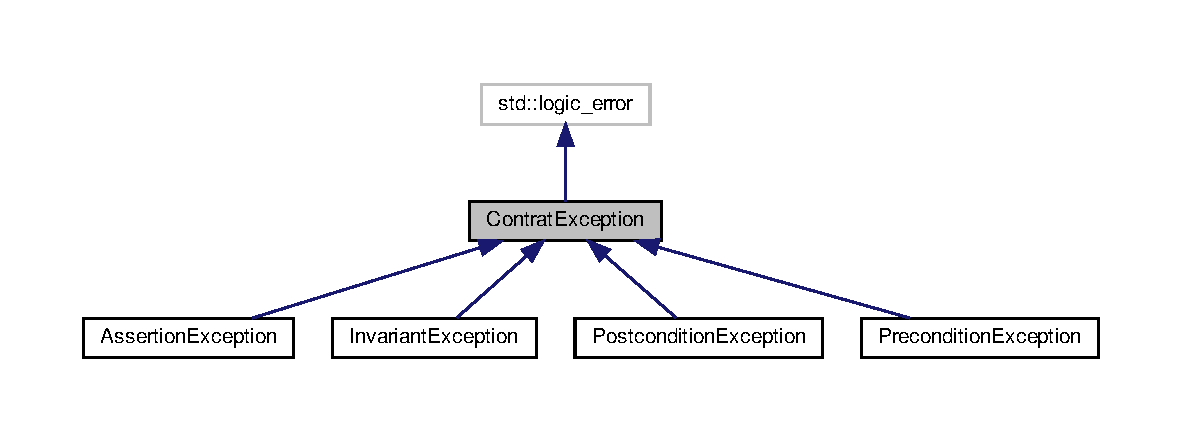
\includegraphics[width=350pt]{classContratException__inherit__graph}
\end{center}
\end{figure}


Collaboration diagram for Contrat\+Exception\+:\nopagebreak
\begin{figure}[H]
\begin{center}
\leavevmode
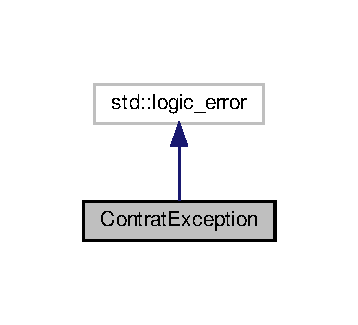
\includegraphics[width=172pt]{classContratException__coll__graph}
\end{center}
\end{figure}
\subsection*{Public Member Functions}
\begin{DoxyCompactItemize}
\item 
\hyperlink{classContratException_ad6c04fb577e960f87e010b125aa636a0}{Contrat\+Exception} (std\+::string, unsigned int, std\+::string, std\+::string)
\begin{DoxyCompactList}\small\item\em Constructeur de la classe de base \hyperlink{classContratException}{Contrat\+Exception}. \end{DoxyCompactList}\item 
std\+::string \hyperlink{classContratException_a59c9ed58985dcdd70af4ee50b2937707}{req\+Texte\+Exception} () const
\begin{DoxyCompactList}\small\item\em Construit le texte complet relié à l\textquotesingle{}exception de contrat. \end{DoxyCompactList}\end{DoxyCompactItemize}


\subsection{Detailed Description}
Classe de base des exceptions de contrat. 

\subsection{Constructor \& Destructor Documentation}
\mbox{\Hypertarget{classContratException_ad6c04fb577e960f87e010b125aa636a0}\label{classContratException_ad6c04fb577e960f87e010b125aa636a0}} 
\index{Contrat\+Exception@{Contrat\+Exception}!Contrat\+Exception@{Contrat\+Exception}}
\index{Contrat\+Exception@{Contrat\+Exception}!Contrat\+Exception@{Contrat\+Exception}}
\subsubsection{\texorpdfstring{Contrat\+Exception()}{ContratException()}}
{\footnotesize\ttfamily Contrat\+Exception\+::\+Contrat\+Exception (\begin{DoxyParamCaption}\item[{std\+::string}]{p\+\_\+fichP,  }\item[{unsigned int}]{p\+\_\+prm\+Ligne,  }\item[{std\+::string}]{p\+\_\+exprP,  }\item[{std\+::string}]{p\+\_\+msgP }\end{DoxyParamCaption})}



Constructeur de la classe de base \hyperlink{classContratException}{Contrat\+Exception}. 


\begin{DoxyParams}{Parameters}
{\em p\+\_\+fichP} & chaîne de caractères représentant le fichier source dans lequel a eu lieu l\textquotesingle{}erreur \\
\hline
{\em p\+\_\+prm\+Ligne} & un entier représentant la ligne où a eu lieu l\textquotesingle{}erreur \\
\hline
{\em p\+\_\+msgP} & Message décrivant l\textquotesingle{}erreur \\
\hline
{\em p\+\_\+exprP} & Test logique qui a échoué \\
\hline
\end{DoxyParams}


\subsection{Member Function Documentation}
\mbox{\Hypertarget{classContratException_a59c9ed58985dcdd70af4ee50b2937707}\label{classContratException_a59c9ed58985dcdd70af4ee50b2937707}} 
\index{Contrat\+Exception@{Contrat\+Exception}!req\+Texte\+Exception@{req\+Texte\+Exception}}
\index{req\+Texte\+Exception@{req\+Texte\+Exception}!Contrat\+Exception@{Contrat\+Exception}}
\subsubsection{\texorpdfstring{req\+Texte\+Exception()}{reqTexteException()}}
{\footnotesize\ttfamily std\+::string Contrat\+Exception\+::req\+Texte\+Exception (\begin{DoxyParamCaption}{ }\end{DoxyParamCaption}) const}



Construit le texte complet relié à l\textquotesingle{}exception de contrat. 

\begin{DoxyReturn}{Returns}
une chaîne de caractères correspondant à l\textquotesingle{}exception 
\end{DoxyReturn}


The documentation for this class was generated from the following files\+:\begin{DoxyCompactItemize}
\item 
\hyperlink{ContratException_8h}{Contrat\+Exception.\+h}\item 
\hyperlink{ContratException_8cpp}{Contrat\+Exception.\+cpp}\end{DoxyCompactItemize}

\hypertarget{classutil_1_1Date}{}\section{util\+:\+:Date Class Reference}
\label{classutil_1_1Date}\index{util\+::\+Date@{util\+::\+Date}}


Cette classe sert au maintien et à la manipulation des dates.  




{\ttfamily \#include $<$Date.\+h$>$}

\subsection*{Public Member Functions}
\begin{DoxyCompactItemize}
\item 
\mbox{\Hypertarget{classutil_1_1Date_a03f7ca00aa80f113bc7c0ebfbd769f54}\label{classutil_1_1Date_a03f7ca00aa80f113bc7c0ebfbd769f54}} 
\hyperlink{classutil_1_1Date_a03f7ca00aa80f113bc7c0ebfbd769f54}{Date} ()
\begin{DoxyCompactList}\small\item\em constructeur par défaut ~\newline
La date prise par défaut est la date du système \end{DoxyCompactList}\item 
\hyperlink{classutil_1_1Date_a06b8340e5beed84c885c89d41a750330}{Date} (long p\+\_\+jour, long p\+\_\+mois, long p\+\_\+annee)
\begin{DoxyCompactList}\small\item\em constructeur avec paramètres On construit un objet \hyperlink{classutil_1_1Date}{Date} à partir de valeurs passées en paramètres. Les attributs sont assignés seulement si la date est considérée comme valide. Autrement, une erreur d\textquotesingle{}assertion est générée. \end{DoxyCompactList}\item 
void \hyperlink{classutil_1_1Date_ab82f59d834f60b929ca130f15e5279c3}{asg\+Date} (long p\+\_\+jour, long p\+\_\+mois, long p\+\_\+annee)
\begin{DoxyCompactList}\small\item\em Assigne une date à l\textquotesingle{}objet courant. \end{DoxyCompactList}\item 
bool \hyperlink{classutil_1_1Date_a7788599612a71d89126d649fdaaced3d}{ajoute\+Nb\+Jour} (long p\+\_\+nbjour)
\begin{DoxyCompactList}\small\item\em Ajoute ou retire un certain nombre de jours à la date courante. \end{DoxyCompactList}\item 
long \hyperlink{classutil_1_1Date_aa2b8c7a6e23e9244a5bac8342484d3b8}{req\+Jour} () const
\begin{DoxyCompactList}\small\item\em retourne le jour de la date \end{DoxyCompactList}\item 
long \hyperlink{classutil_1_1Date_a8002c391b812945da68b16cb4a424460}{req\+Mois} () const
\begin{DoxyCompactList}\small\item\em retourne le mois de la date \end{DoxyCompactList}\item 
long \hyperlink{classutil_1_1Date_aa7c4b428456da55a2e3769e93ad9bb8d}{req\+Annee} () const
\begin{DoxyCompactList}\small\item\em retourne l\textquotesingle{}année de la date \end{DoxyCompactList}\item 
long \hyperlink{classutil_1_1Date_a9e76af410b6be9ac4ea9ab4df5797847}{req\+Jour\+Annee} () const
\begin{DoxyCompactList}\small\item\em retourne le ième jour de l\textquotesingle{}année correspondant au jour de la date \end{DoxyCompactList}\item 
std\+::string \hyperlink{classutil_1_1Date_ad92d1e9c4d570c5f31a8e06cf2e1ae8c}{req\+Date\+Formatee} () const
\begin{DoxyCompactList}\small\item\em retourne une date formatée dans une chaîne de caracères (string) \end{DoxyCompactList}\item 
bool \hyperlink{classutil_1_1Date_a8114f8e40cee24e1d7a58b910e8f4637}{operator==} (const \hyperlink{classutil_1_1Date}{Date} \&p\+\_\+date) const
\begin{DoxyCompactList}\small\item\em surcharge de l\textquotesingle{}opérateur == \end{DoxyCompactList}\item 
bool \hyperlink{classutil_1_1Date_aefcf8a7520711f783fb0241d460480c5}{operator$<$} (const \hyperlink{classutil_1_1Date}{Date} \&p\+\_\+date) const
\begin{DoxyCompactList}\small\item\em surcharge de l\textquotesingle{}opérateur $<$ \end{DoxyCompactList}\item 
int \hyperlink{classutil_1_1Date_af12f2c545070b5e2b397be5379c5c3fd}{operator-\/} (const \hyperlink{classutil_1_1Date}{Date} \&p\+\_\+date) const
\begin{DoxyCompactList}\small\item\em retourne le nombre de jours entre deux dates \end{DoxyCompactList}\end{DoxyCompactItemize}
\subsection*{Static Public Member Functions}
\begin{DoxyCompactItemize}
\item 
static bool \hyperlink{classutil_1_1Date_af80efec6a713cdb671d8b23c3e8c4efb}{est\+Bissextile} (long p\+\_\+annee)
\begin{DoxyCompactList}\small\item\em Déterminer si une année est bissextile ou non. \end{DoxyCompactList}\item 
static bool \hyperlink{classutil_1_1Date_af4b4dde01395754245a42483358cb538}{valider\+Date} (long p\+\_\+jour, long p\+\_\+mois, long p\+\_\+annee)
\begin{DoxyCompactList}\small\item\em Vérifie la validité d\textquotesingle{}une date. \end{DoxyCompactList}\end{DoxyCompactItemize}
\subsection*{Friends}
\begin{DoxyCompactItemize}
\item 
\mbox{\Hypertarget{classutil_1_1Date_ab01372aff5a2aa1d5f5bab251bb7951c}\label{classutil_1_1Date_ab01372aff5a2aa1d5f5bab251bb7951c}} 
std\+::ostream \& {\bfseries operator$<$$<$} (std\+::ostream \&p\+\_\+os, const \hyperlink{classutil_1_1Date}{Date} \&p\+\_\+date)
\end{DoxyCompactItemize}
\subsection*{Related Functions}
(Note that these are not member functions.) \begin{DoxyCompactItemize}
\item 
ostream \& \hyperlink{classutil_1_1Date_a3b88f9a1692395518a45b282a19f10e8}{operator$<$$<$} (ostream \&p\+\_\+os, const \hyperlink{classutil_1_1Date}{Date} \&p\+\_\+date)
\begin{DoxyCompactList}\small\item\em surcharge de la fonction $<$$<$ d\textquotesingle{}écriture dans un flux de sortie \end{DoxyCompactList}\end{DoxyCompactItemize}


\subsection{Detailed Description}
Cette classe sert au maintien et à la manipulation des dates. 

La classe maintient dans un état cohérent ces renseignements. Elle valide ce qu\textquotesingle{}on veut lui assigner. 

Cette classe peut aussi servir à prendre la date courante du système et à faire des calculs avec des dates. 

La classe n\textquotesingle{}accepte que des dates valides, c\textquotesingle{}est la responsabilité de l\textquotesingle{}utilisateur de la classe de s\textquotesingle{}en assurer. 

Attributs\+: time\+\_\+t m\+\_\+temps Nombre de secondes écoulé depuis le premier janvier 1970 

time\+\_\+t m\+\_\+temps pour long m\+\_\+temps \begin{DoxyInvariant}{Invariant}
m\+\_\+temps $>$= 1er janvier 1970 et $>$= au 31 décembre 2037 

La validité peut être vérifiée avec la méthode statique bool Date\+::verifier\+Date(jour, mois, annee). 
\end{DoxyInvariant}


\subsection{Constructor \& Destructor Documentation}
\mbox{\Hypertarget{classutil_1_1Date_a06b8340e5beed84c885c89d41a750330}\label{classutil_1_1Date_a06b8340e5beed84c885c89d41a750330}} 
\index{util\+::\+Date@{util\+::\+Date}!Date@{Date}}
\index{Date@{Date}!util\+::\+Date@{util\+::\+Date}}
\subsubsection{\texorpdfstring{Date()}{Date()}}
{\footnotesize\ttfamily util\+::\+Date\+::\+Date (\begin{DoxyParamCaption}\item[{long}]{p\+\_\+jour,  }\item[{long}]{p\+\_\+mois,  }\item[{long}]{p\+\_\+annee }\end{DoxyParamCaption})}



constructeur avec paramètres On construit un objet \hyperlink{classutil_1_1Date}{Date} à partir de valeurs passées en paramètres. Les attributs sont assignés seulement si la date est considérée comme valide. Autrement, une erreur d\textquotesingle{}assertion est générée. 


\begin{DoxyParams}[1]{Parameters}
\mbox{\tt in}  & {\em p\+\_\+jour} & est un entier long qui représente le jour de la date \\
\hline
\mbox{\tt in}  & {\em p\+\_\+mois} & est un entier long qui représente le mois de la date \\
\hline
\mbox{\tt in}  & {\em p\+\_\+annee} & est un entier long qui représente l\textquotesingle{}année de la date \\
\hline
\end{DoxyParams}
\begin{DoxyPrecond}{Precondition}
p\+\_\+jour, p\+\_\+mois, p\+\_\+annee doivent correspondre à une date valide 
\end{DoxyPrecond}
\begin{DoxyPostcond}{Postcondition}
l\textquotesingle{}objet construit a été initialisé à partir des entiers passés en paramètres 
\end{DoxyPostcond}


\subsection{Member Function Documentation}
\mbox{\Hypertarget{classutil_1_1Date_a7788599612a71d89126d649fdaaced3d}\label{classutil_1_1Date_a7788599612a71d89126d649fdaaced3d}} 
\index{util\+::\+Date@{util\+::\+Date}!ajoute\+Nb\+Jour@{ajoute\+Nb\+Jour}}
\index{ajoute\+Nb\+Jour@{ajoute\+Nb\+Jour}!util\+::\+Date@{util\+::\+Date}}
\subsubsection{\texorpdfstring{ajoute\+Nb\+Jour()}{ajouteNbJour()}}
{\footnotesize\ttfamily bool util\+::\+Date\+::ajoute\+Nb\+Jour (\begin{DoxyParamCaption}\item[{long}]{p\+\_\+nb\+Jour }\end{DoxyParamCaption})}



Ajoute ou retire un certain nombre de jours à la date courante. 


\begin{DoxyParams}{Parameters}
{\em p\+\_\+nb\+Jour} & est une entier long qui représente le nombre de jours à ajouter ou à soustraire s\textquotesingle{}il est négatif \\
\hline
\end{DoxyParams}
\begin{DoxyReturn}{Returns}
un booléen qui indique si l\textquotesingle{}opération a réussi ou non 
\end{DoxyReturn}
\mbox{\Hypertarget{classutil_1_1Date_ab82f59d834f60b929ca130f15e5279c3}\label{classutil_1_1Date_ab82f59d834f60b929ca130f15e5279c3}} 
\index{util\+::\+Date@{util\+::\+Date}!asg\+Date@{asg\+Date}}
\index{asg\+Date@{asg\+Date}!util\+::\+Date@{util\+::\+Date}}
\subsubsection{\texorpdfstring{asg\+Date()}{asgDate()}}
{\footnotesize\ttfamily void util\+::\+Date\+::asg\+Date (\begin{DoxyParamCaption}\item[{long}]{p\+\_\+jour,  }\item[{long}]{p\+\_\+mois,  }\item[{long}]{p\+\_\+annee }\end{DoxyParamCaption})}



Assigne une date à l\textquotesingle{}objet courant. 


\begin{DoxyParams}[1]{Parameters}
\mbox{\tt in}  & {\em p\+\_\+jour} & est un entier long qui représente le jour de la date \\
\hline
\mbox{\tt in}  & {\em p\+\_\+mois} & est un entier long qui représente le mois de la date \\
\hline
\mbox{\tt in}  & {\em p\+\_\+annee} & est un entier long qui représente l\textquotesingle{}année de la date \\
\hline
\end{DoxyParams}
\begin{DoxyPrecond}{Precondition}
p\+\_\+jour, p\+\_\+mois, p\+\_\+annee doivent correspondre à une date valide 
\end{DoxyPrecond}
\begin{DoxyPostcond}{Postcondition}
l\textquotesingle{}objet a été assigné à partir des entiers passés en paramètres 
\end{DoxyPostcond}
\mbox{\Hypertarget{classutil_1_1Date_af80efec6a713cdb671d8b23c3e8c4efb}\label{classutil_1_1Date_af80efec6a713cdb671d8b23c3e8c4efb}} 
\index{util\+::\+Date@{util\+::\+Date}!est\+Bissextile@{est\+Bissextile}}
\index{est\+Bissextile@{est\+Bissextile}!util\+::\+Date@{util\+::\+Date}}
\subsubsection{\texorpdfstring{est\+Bissextile()}{estBissextile()}}
{\footnotesize\ttfamily bool util\+::\+Date\+::est\+Bissextile (\begin{DoxyParamCaption}\item[{long}]{p\+\_\+annee }\end{DoxyParamCaption})\hspace{0.3cm}{\ttfamily [static]}}



Déterminer si une année est bissextile ou non. 


\begin{DoxyParams}[1]{Parameters}
\mbox{\tt in}  & {\em p\+\_\+annee} & un entier long qui représente l\textquotesingle{}année à vérifier \\
\hline
\end{DoxyParams}
\begin{DoxyReturn}{Returns}
est\+Bissextile un booléen qui a la valeur true si l\textquotesingle{}année est bissextile et false sinon 
\end{DoxyReturn}
\mbox{\Hypertarget{classutil_1_1Date_af12f2c545070b5e2b397be5379c5c3fd}\label{classutil_1_1Date_af12f2c545070b5e2b397be5379c5c3fd}} 
\index{util\+::\+Date@{util\+::\+Date}!operator-\/@{operator-\/}}
\index{operator-\/@{operator-\/}!util\+::\+Date@{util\+::\+Date}}
\subsubsection{\texorpdfstring{operator-\/()}{operator-()}}
{\footnotesize\ttfamily int util\+::\+Date\+::operator-\/ (\begin{DoxyParamCaption}\item[{const \hyperlink{classutil_1_1Date}{Date} \&}]{p\+\_\+date }\end{DoxyParamCaption}) const}



retourne le nombre de jours entre deux dates 


\begin{DoxyParams}[1]{Parameters}
\mbox{\tt in}  & {\em p\+\_\+date} & à soustraire à la date courante \\
\hline
\end{DoxyParams}
\begin{DoxyReturn}{Returns}
un entier qui représente le nombre de jours entre la date courante et celle passée en paramètre 
\end{DoxyReturn}
\mbox{\Hypertarget{classutil_1_1Date_aefcf8a7520711f783fb0241d460480c5}\label{classutil_1_1Date_aefcf8a7520711f783fb0241d460480c5}} 
\index{util\+::\+Date@{util\+::\+Date}!operator$<$@{operator$<$}}
\index{operator$<$@{operator$<$}!util\+::\+Date@{util\+::\+Date}}
\subsubsection{\texorpdfstring{operator$<$()}{operator<()}}
{\footnotesize\ttfamily bool util\+::\+Date\+::operator$<$ (\begin{DoxyParamCaption}\item[{const \hyperlink{classutil_1_1Date}{Date} \&}]{p\+\_\+date }\end{DoxyParamCaption}) const}



surcharge de l\textquotesingle{}opérateur $<$ 


\begin{DoxyParams}[1]{Parameters}
\mbox{\tt in}  & {\em p\+\_\+date} & à comparer à la date courante \\
\hline
\end{DoxyParams}
\begin{DoxyReturn}{Returns}
un booléen indiquant si la date courante est plus petite que la date passée en paramètre 
\end{DoxyReturn}
\mbox{\Hypertarget{classutil_1_1Date_a8114f8e40cee24e1d7a58b910e8f4637}\label{classutil_1_1Date_a8114f8e40cee24e1d7a58b910e8f4637}} 
\index{util\+::\+Date@{util\+::\+Date}!operator==@{operator==}}
\index{operator==@{operator==}!util\+::\+Date@{util\+::\+Date}}
\subsubsection{\texorpdfstring{operator==()}{operator==()}}
{\footnotesize\ttfamily bool util\+::\+Date\+::operator== (\begin{DoxyParamCaption}\item[{const \hyperlink{classutil_1_1Date}{Date} \&}]{p\+\_\+date }\end{DoxyParamCaption}) const}



surcharge de l\textquotesingle{}opérateur == 


\begin{DoxyParams}[1]{Parameters}
\mbox{\tt in}  & {\em p\+\_\+date} & à comparer à la date courante \\
\hline
\end{DoxyParams}
\begin{DoxyReturn}{Returns}
un booléen indiquant si les deux dates sont égales ou non 
\end{DoxyReturn}
\mbox{\Hypertarget{classutil_1_1Date_aa7c4b428456da55a2e3769e93ad9bb8d}\label{classutil_1_1Date_aa7c4b428456da55a2e3769e93ad9bb8d}} 
\index{util\+::\+Date@{util\+::\+Date}!req\+Annee@{req\+Annee}}
\index{req\+Annee@{req\+Annee}!util\+::\+Date@{util\+::\+Date}}
\subsubsection{\texorpdfstring{req\+Annee()}{reqAnnee()}}
{\footnotesize\ttfamily long util\+::\+Date\+::req\+Annee (\begin{DoxyParamCaption}{ }\end{DoxyParamCaption}) const}



retourne l\textquotesingle{}année de la date 

\begin{DoxyReturn}{Returns}
un entier long qui représente l\textquotesingle{}année de la date 
\end{DoxyReturn}
\mbox{\Hypertarget{classutil_1_1Date_ad92d1e9c4d570c5f31a8e06cf2e1ae8c}\label{classutil_1_1Date_ad92d1e9c4d570c5f31a8e06cf2e1ae8c}} 
\index{util\+::\+Date@{util\+::\+Date}!req\+Date\+Formatee@{req\+Date\+Formatee}}
\index{req\+Date\+Formatee@{req\+Date\+Formatee}!util\+::\+Date@{util\+::\+Date}}
\subsubsection{\texorpdfstring{req\+Date\+Formatee()}{reqDateFormatee()}}
{\footnotesize\ttfamily string util\+::\+Date\+::req\+Date\+Formatee (\begin{DoxyParamCaption}{ }\end{DoxyParamCaption}) const}



retourne une date formatée dans une chaîne de caracères (string) 

\begin{DoxyReturn}{Returns}
la date formatée dans une chaîne de caractères 
\end{DoxyReturn}
\mbox{\Hypertarget{classutil_1_1Date_aa2b8c7a6e23e9244a5bac8342484d3b8}\label{classutil_1_1Date_aa2b8c7a6e23e9244a5bac8342484d3b8}} 
\index{util\+::\+Date@{util\+::\+Date}!req\+Jour@{req\+Jour}}
\index{req\+Jour@{req\+Jour}!util\+::\+Date@{util\+::\+Date}}
\subsubsection{\texorpdfstring{req\+Jour()}{reqJour()}}
{\footnotesize\ttfamily long util\+::\+Date\+::req\+Jour (\begin{DoxyParamCaption}{ }\end{DoxyParamCaption}) const}



retourne le jour de la date 

\begin{DoxyReturn}{Returns}
un entier long qui représente le jour de la date 
\end{DoxyReturn}
\mbox{\Hypertarget{classutil_1_1Date_a9e76af410b6be9ac4ea9ab4df5797847}\label{classutil_1_1Date_a9e76af410b6be9ac4ea9ab4df5797847}} 
\index{util\+::\+Date@{util\+::\+Date}!req\+Jour\+Annee@{req\+Jour\+Annee}}
\index{req\+Jour\+Annee@{req\+Jour\+Annee}!util\+::\+Date@{util\+::\+Date}}
\subsubsection{\texorpdfstring{req\+Jour\+Annee()}{reqJourAnnee()}}
{\footnotesize\ttfamily long util\+::\+Date\+::req\+Jour\+Annee (\begin{DoxyParamCaption}{ }\end{DoxyParamCaption}) const}



retourne le ième jour de l\textquotesingle{}année correspondant au jour de la date 

\begin{DoxyReturn}{Returns}
un entier long qui représente le ième jour de l\textquotesingle{}année 
\end{DoxyReturn}
\mbox{\Hypertarget{classutil_1_1Date_a8002c391b812945da68b16cb4a424460}\label{classutil_1_1Date_a8002c391b812945da68b16cb4a424460}} 
\index{util\+::\+Date@{util\+::\+Date}!req\+Mois@{req\+Mois}}
\index{req\+Mois@{req\+Mois}!util\+::\+Date@{util\+::\+Date}}
\subsubsection{\texorpdfstring{req\+Mois()}{reqMois()}}
{\footnotesize\ttfamily long util\+::\+Date\+::req\+Mois (\begin{DoxyParamCaption}{ }\end{DoxyParamCaption}) const}



retourne le mois de la date 

\begin{DoxyReturn}{Returns}
un entier long qui représente le mois de la date 
\end{DoxyReturn}
\mbox{\Hypertarget{classutil_1_1Date_af4b4dde01395754245a42483358cb538}\label{classutil_1_1Date_af4b4dde01395754245a42483358cb538}} 
\index{util\+::\+Date@{util\+::\+Date}!valider\+Date@{valider\+Date}}
\index{valider\+Date@{valider\+Date}!util\+::\+Date@{util\+::\+Date}}
\subsubsection{\texorpdfstring{valider\+Date()}{validerDate()}}
{\footnotesize\ttfamily bool util\+::\+Date\+::valider\+Date (\begin{DoxyParamCaption}\item[{long}]{p\+\_\+jour,  }\item[{long}]{p\+\_\+mois,  }\item[{long}]{p\+\_\+annee }\end{DoxyParamCaption})\hspace{0.3cm}{\ttfamily [static]}}



Vérifie la validité d\textquotesingle{}une date. 


\begin{DoxyParams}[1]{Parameters}
\mbox{\tt in}  & {\em p\+\_\+jour} & un entier long représentant le jour de la date \\
\hline
\mbox{\tt in}  & {\em p\+\_\+mois} & un entier long représentant le mois de la date \\
\hline
\mbox{\tt in}  & {\em p\+\_\+annee} & un entier long représentant l\textquotesingle{}année de la date \\
\hline
\end{DoxyParams}
\begin{DoxyReturn}{Returns}
un booléen indiquant si la date est valide ou non 
\end{DoxyReturn}


\subsection{Friends And Related Function Documentation}
\mbox{\Hypertarget{classutil_1_1Date_a3b88f9a1692395518a45b282a19f10e8}\label{classutil_1_1Date_a3b88f9a1692395518a45b282a19f10e8}} 
\index{util\+::\+Date@{util\+::\+Date}!operator$<$$<$@{operator$<$$<$}}
\index{operator$<$$<$@{operator$<$$<$}!util\+::\+Date@{util\+::\+Date}}
\subsubsection{\texorpdfstring{operator$<$$<$()}{operator<<()}}
{\footnotesize\ttfamily ostream \& operator$<$$<$ (\begin{DoxyParamCaption}\item[{ostream \&}]{p\+\_\+os,  }\item[{const \hyperlink{classutil_1_1Date}{Date} \&}]{p\+\_\+date }\end{DoxyParamCaption})\hspace{0.3cm}{\ttfamily [related]}}



surcharge de la fonction $<$$<$ d\textquotesingle{}écriture dans un flux de sortie 


\begin{DoxyParams}[1]{Parameters}
\mbox{\tt in}  & {\em p\+\_\+os} & un flux de sortie dans laquelle on va écrire \\
\hline
\mbox{\tt in}  & {\em p\+\_\+date} & sortie dans le flux \\
\hline
\end{DoxyParams}
\begin{DoxyReturn}{Returns}
le flux dans lequel on a écrit la date, ceci pour les appels en cascade 
\end{DoxyReturn}


The documentation for this class was generated from the following files\+:\begin{DoxyCompactItemize}
\item 
\hyperlink{Date_8h}{Date.\+h}\item 
\hyperlink{Date_8cpp}{Date.\+cpp}\end{DoxyCompactItemize}

\hypertarget{classelections_1_1Electeur}{}\section{elections\+:\+:Electeur Class Reference}
\label{classelections_1_1Electeur}\index{elections\+::\+Electeur@{elections\+::\+Electeur}}


Classe dérivée de la classe \hyperlink{classelections_1_1Personne}{Personne}.  




{\ttfamily \#include $<$Electeur.\+h$>$}



Inheritance diagram for elections\+:\+:Electeur\+:\nopagebreak
\begin{figure}[H]
\begin{center}
\leavevmode
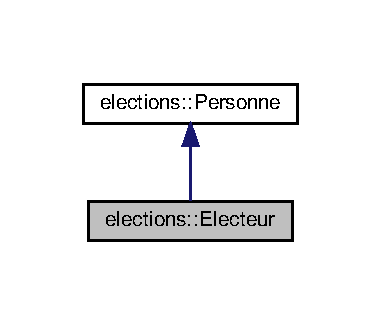
\includegraphics[width=183pt]{classelections_1_1Electeur__inherit__graph}
\end{center}
\end{figure}


Collaboration diagram for elections\+:\+:Electeur\+:\nopagebreak
\begin{figure}[H]
\begin{center}
\leavevmode
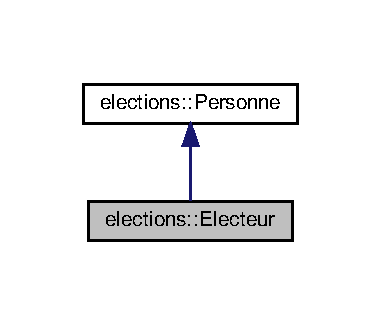
\includegraphics[width=183pt]{classelections_1_1Electeur__coll__graph}
\end{center}
\end{figure}
\subsection*{Public Member Functions}
\begin{DoxyCompactItemize}
\item 
\hyperlink{classelections_1_1Electeur_acaa3408d3c2556b55d3f1bb880edfd19}{Electeur} (const string \&p\+\_\+nas, const string \&p\+\_\+prenom, const string \&p\+\_\+nom, const \hyperlink{classutil_1_1Date}{util\+::\+Date} \&p\+\_\+date\+Naissance, const \hyperlink{classutil_1_1Adresse}{util\+::\+Adresse} \&p\+\_\+adresse)
\begin{DoxyCompactList}\small\item\em Constructeur avec paramètres Création d\textquotesingle{}un objet \hyperlink{classelections_1_1Electeur}{Electeur} à partir de valeurs passées en paramètres. \end{DoxyCompactList}\item 
virtual \hyperlink{classelections_1_1Personne}{Personne} $\ast$ \hyperlink{classelections_1_1Electeur_a948f48b32633f91670b3b0fde9dff3a4}{clone} () const
\begin{DoxyCompactList}\small\item\em \hyperlink{classelections_1_1Electeur_a948f48b32633f91670b3b0fde9dff3a4}{clone()} permet de faire une copie allouée sur le monceau de l\textquotesingle{}objet courant \end{DoxyCompactList}\item 
virtual std\+::string \hyperlink{classelections_1_1Electeur_ac233f4fb12d9267374c8e66864d89689}{req\+Personne\+Formate} () const
\begin{DoxyCompactList}\small\item\em Affiche les informations de l\textquotesingle{}electeur sous forme d\textquotesingle{}une chaîne de caractère formatée. \end{DoxyCompactList}\end{DoxyCompactItemize}


\subsection{Detailed Description}
Classe dérivée de la classe \hyperlink{classelections_1_1Personne}{Personne}. 

\subsection{Constructor \& Destructor Documentation}
\mbox{\Hypertarget{classelections_1_1Electeur_acaa3408d3c2556b55d3f1bb880edfd19}\label{classelections_1_1Electeur_acaa3408d3c2556b55d3f1bb880edfd19}} 
\index{elections\+::\+Electeur@{elections\+::\+Electeur}!Electeur@{Electeur}}
\index{Electeur@{Electeur}!elections\+::\+Electeur@{elections\+::\+Electeur}}
\subsubsection{\texorpdfstring{Electeur()}{Electeur()}}
{\footnotesize\ttfamily elections\+::\+Electeur\+::\+Electeur (\begin{DoxyParamCaption}\item[{const string \&}]{p\+\_\+nas,  }\item[{const string \&}]{p\+\_\+prenom,  }\item[{const string \&}]{p\+\_\+nom,  }\item[{const \hyperlink{classutil_1_1Date}{util\+::\+Date} \&}]{p\+\_\+date\+Naissance,  }\item[{const \hyperlink{classutil_1_1Adresse}{util\+::\+Adresse} \&}]{p\+\_\+adresse }\end{DoxyParamCaption})}



Constructeur avec paramètres Création d\textquotesingle{}un objet \hyperlink{classelections_1_1Electeur}{Electeur} à partir de valeurs passées en paramètres. 


\begin{DoxyParams}[1]{Parameters}
\mbox{\tt in}  & {\em p\+\_\+nas} & nas de l\textquotesingle{}electeur \\
\hline
\mbox{\tt in}  & {\em p\+\_\+prenom} & prenom de l\textquotesingle{}electeur \\
\hline
\mbox{\tt in}  & {\em p\+\_\+nom} & nom de l\textquotesingle{}electeur \\
\hline
\mbox{\tt in}  & {\em p\+\_\+date\+Naissance} & date de naissance de l\textquotesingle{}electeur \\
\hline
\mbox{\tt in}  & {\em p\+\_\+adresse} & adresse de l\textquotesingle{}electeur \\
\hline
\end{DoxyParams}


\subsection{Member Function Documentation}
\mbox{\Hypertarget{classelections_1_1Electeur_a948f48b32633f91670b3b0fde9dff3a4}\label{classelections_1_1Electeur_a948f48b32633f91670b3b0fde9dff3a4}} 
\index{elections\+::\+Electeur@{elections\+::\+Electeur}!clone@{clone}}
\index{clone@{clone}!elections\+::\+Electeur@{elections\+::\+Electeur}}
\subsubsection{\texorpdfstring{clone()}{clone()}}
{\footnotesize\ttfamily \hyperlink{classelections_1_1Personne}{Personne} $\ast$ elections\+::\+Electeur\+::clone (\begin{DoxyParamCaption}{ }\end{DoxyParamCaption}) const\hspace{0.3cm}{\ttfamily [virtual]}}



\hyperlink{classelections_1_1Electeur_a948f48b32633f91670b3b0fde9dff3a4}{clone()} permet de faire une copie allouée sur le monceau de l\textquotesingle{}objet courant 

\begin{DoxyReturn}{Returns}
pointeur d’electeur 
\end{DoxyReturn}


Implements \hyperlink{classelections_1_1Personne}{elections\+::\+Personne}.

\mbox{\Hypertarget{classelections_1_1Electeur_ac233f4fb12d9267374c8e66864d89689}\label{classelections_1_1Electeur_ac233f4fb12d9267374c8e66864d89689}} 
\index{elections\+::\+Electeur@{elections\+::\+Electeur}!req\+Personne\+Formate@{req\+Personne\+Formate}}
\index{req\+Personne\+Formate@{req\+Personne\+Formate}!elections\+::\+Electeur@{elections\+::\+Electeur}}
\subsubsection{\texorpdfstring{req\+Personne\+Formate()}{reqPersonneFormate()}}
{\footnotesize\ttfamily string elections\+::\+Electeur\+::req\+Personne\+Formate (\begin{DoxyParamCaption}{ }\end{DoxyParamCaption}) const\hspace{0.3cm}{\ttfamily [virtual]}}



Affiche les informations de l\textquotesingle{}electeur sous forme d\textquotesingle{}une chaîne de caractère formatée. 

\begin{DoxyReturn}{Returns}
les informations sur un electeur 
\end{DoxyReturn}


Implements \hyperlink{classelections_1_1Personne_aac1232e61b7cb9743bafba9280041d35}{elections\+::\+Personne}.



The documentation for this class was generated from the following files\+:\begin{DoxyCompactItemize}
\item 
\hyperlink{Electeur_8h}{Electeur.\+h}\item 
\hyperlink{Electeur_8cpp}{Electeur.\+cpp}\end{DoxyCompactItemize}

\hypertarget{classInvariantException}{}\section{Invariant\+Exception Class Reference}
\label{classInvariantException}\index{Invariant\+Exception@{Invariant\+Exception}}


Classe pour la gestion des erreurs d\textquotesingle{}invariant.  




{\ttfamily \#include $<$Contrat\+Exception.\+h$>$}



Inheritance diagram for Invariant\+Exception\+:\nopagebreak
\begin{figure}[H]
\begin{center}
\leavevmode
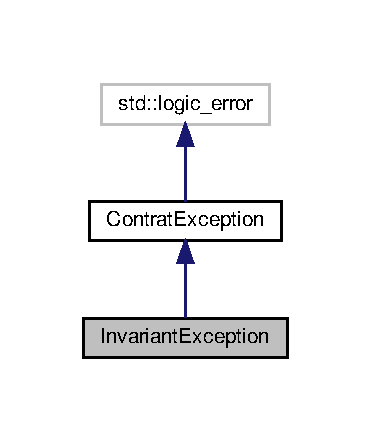
\includegraphics[width=178pt]{classInvariantException__inherit__graph}
\end{center}
\end{figure}


Collaboration diagram for Invariant\+Exception\+:\nopagebreak
\begin{figure}[H]
\begin{center}
\leavevmode
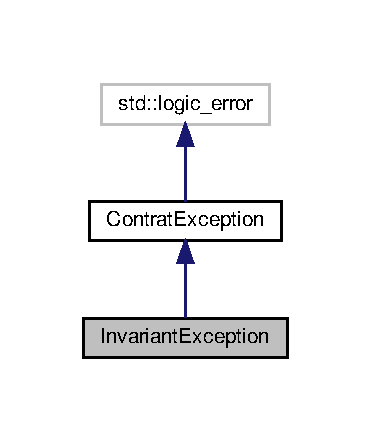
\includegraphics[width=178pt]{classInvariantException__coll__graph}
\end{center}
\end{figure}
\subsection*{Public Member Functions}
\begin{DoxyCompactItemize}
\item 
\hyperlink{classInvariantException_af8a1950834b26c256db0b11eb33e6056}{Invariant\+Exception} (std\+::string, unsigned int, std\+::string)
\begin{DoxyCompactList}\small\item\em Constructeur de la classe \hyperlink{classInvariantException}{Invariant\+Exception} en initialisant la classe de base \hyperlink{classContratException}{Contrat\+Exception}. La classe représente des erreurs d\textquotesingle{}invariant dans la théorie du contrat. \end{DoxyCompactList}\end{DoxyCompactItemize}


\subsection{Detailed Description}
Classe pour la gestion des erreurs d\textquotesingle{}invariant. 

\subsection{Constructor \& Destructor Documentation}
\mbox{\Hypertarget{classInvariantException_af8a1950834b26c256db0b11eb33e6056}\label{classInvariantException_af8a1950834b26c256db0b11eb33e6056}} 
\index{Invariant\+Exception@{Invariant\+Exception}!Invariant\+Exception@{Invariant\+Exception}}
\index{Invariant\+Exception@{Invariant\+Exception}!Invariant\+Exception@{Invariant\+Exception}}
\subsubsection{\texorpdfstring{Invariant\+Exception()}{InvariantException()}}
{\footnotesize\ttfamily Invariant\+Exception\+::\+Invariant\+Exception (\begin{DoxyParamCaption}\item[{std\+::string}]{p\+\_\+fichP,  }\item[{unsigned int}]{p\+\_\+prm\+Ligne,  }\item[{std\+::string}]{p\+\_\+exprP }\end{DoxyParamCaption})}



Constructeur de la classe \hyperlink{classInvariantException}{Invariant\+Exception} en initialisant la classe de base \hyperlink{classContratException}{Contrat\+Exception}. La classe représente des erreurs d\textquotesingle{}invariant dans la théorie du contrat. 


\begin{DoxyParams}{Parameters}
{\em p\+\_\+fichP} & chaîne de caractères représentant le fichier source dans lequel a eu lieu l\textquotesingle{}erreur \\
\hline
{\em p\+\_\+prm\+Ligne} & un entier représentant la ligne où a eu lieu l\textquotesingle{}erreur \\
\hline
{\em p\+\_\+exprP} & Test logique qui a échoué \\
\hline
\end{DoxyParams}


The documentation for this class was generated from the following files\+:\begin{DoxyCompactItemize}
\item 
\hyperlink{ContratException_8h}{Contrat\+Exception.\+h}\item 
\hyperlink{ContratException_8cpp}{Contrat\+Exception.\+cpp}\end{DoxyCompactItemize}

\hypertarget{classelections_1_1Personne}{}\section{elections\+:\+:Personne Class Reference}
\label{classelections_1_1Personne}\index{elections\+::\+Personne@{elections\+::\+Personne}}


Cette classe sert au maintien et à la manipulation des informations sur une personne. La classe \hyperlink{classelections_1_1Personne}{Personne} permet d\textquotesingle{}implanter des personnes.  




{\ttfamily \#include $<$Personne.\+h$>$}



Inheritance diagram for elections\+:\+:Personne\+:\nopagebreak
\begin{figure}[H]
\begin{center}
\leavevmode
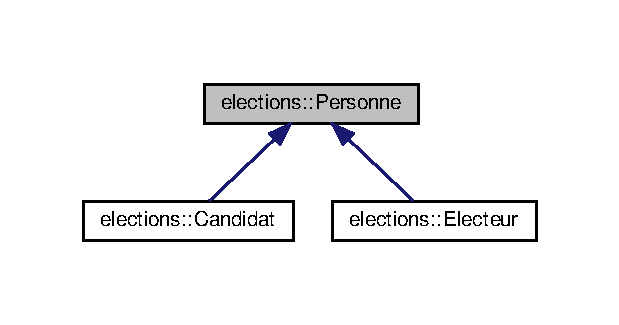
\includegraphics[width=297pt]{classelections_1_1Personne__inherit__graph}
\end{center}
\end{figure}
\subsection*{Public Member Functions}
\begin{DoxyCompactItemize}
\item 
\hyperlink{classelections_1_1Personne_a25e4a5ff2a6b2fd79d146510b0d4622f}{Personne} (const std\+::string \&p\+\_\+nas, const std\+::string \&p\+\_\+prenom, const std\+::string \&p\+\_\+nom, const \hyperlink{classutil_1_1Date}{util\+::\+Date} \&p\+\_\+date\+Naissance, const \hyperlink{classutil_1_1Adresse}{util\+::\+Adresse} \&p\+\_\+adresse)
\begin{DoxyCompactList}\small\item\em constructeur avec paramètres On construit un objet \hyperlink{classelections_1_1Personne}{Personne} à partir de valeurs passées en paramètres. \end{DoxyCompactList}\item 
\mbox{\Hypertarget{classelections_1_1Personne_a5797ace33d89a69dcc87420833affa3a}\label{classelections_1_1Personne_a5797ace33d89a69dcc87420833affa3a}} 
virtual \hyperlink{classelections_1_1Personne}{Personne} $\ast$ {\bfseries clone} () const =0
\item 
const std\+::string \& \hyperlink{classelections_1_1Personne_af822cf5097138148a8ecdc4312521743}{req\+Nas} () const
\begin{DoxyCompactList}\small\item\em retourne le nas d\textquotesingle{}une personne \end{DoxyCompactList}\item 
const std\+::string \& \hyperlink{classelections_1_1Personne_a308b2c6b55cf3d0f414ba5c19873169f}{req\+Prenom} () const
\begin{DoxyCompactList}\small\item\em retourne le prenom d\textquotesingle{}une personne \end{DoxyCompactList}\item 
const std\+::string \& \hyperlink{classelections_1_1Personne_a46cfdb57aa5d46c54b3a8c2860ca2e30}{req\+Nom} () const
\begin{DoxyCompactList}\small\item\em retourne le nom d\textquotesingle{}une personne \end{DoxyCompactList}\item 
const \hyperlink{classutil_1_1Date}{util\+::\+Date} \& \hyperlink{classelections_1_1Personne_a32ff2a825ffb56f8159b6b618a8c897d}{req\+Date\+Naissance} () const
\begin{DoxyCompactList}\small\item\em retourne la date de naissance d\textquotesingle{}une personne \end{DoxyCompactList}\item 
const \hyperlink{classutil_1_1Adresse}{util\+::\+Adresse} \& \hyperlink{classelections_1_1Personne_a908c8e2362d6b3bbbc6c24f8f7a4e460}{req\+Adresse} () const
\begin{DoxyCompactList}\small\item\em retourne l\textquotesingle{}adresse d\textquotesingle{}une personne \end{DoxyCompactList}\item 
void \hyperlink{classelections_1_1Personne_a1aeeb0241c9065cb43a0393f7dc1d26c}{asg\+Nouvelle\+Adresse} (const \hyperlink{classutil_1_1Adresse}{util\+::\+Adresse} \&p\+\_\+adresse)
\begin{DoxyCompactList}\small\item\em Assigne une \hyperlink{classelections_1_1Personne}{Personne} à l\textquotesingle{}objet courant. \end{DoxyCompactList}\item 
bool \hyperlink{classelections_1_1Personne_a991bb78bcf3a7ea7574d7d991c7595d9}{operator==} (const \hyperlink{classelections_1_1Personne}{Personne} \&p\+\_\+personne) const
\begin{DoxyCompactList}\small\item\em surcharge de l\textquotesingle{}opérateur == \end{DoxyCompactList}\item 
virtual std\+::string \hyperlink{classelections_1_1Personne_aac1232e61b7cb9743bafba9280041d35}{req\+Personne\+Formate} () const =0
\begin{DoxyCompactList}\small\item\em retourne une personne formatée dans une chaîne de caractères (string) \end{DoxyCompactList}\end{DoxyCompactItemize}


\subsection{Detailed Description}
Cette classe sert au maintien et à la manipulation des informations sur une personne. La classe \hyperlink{classelections_1_1Personne}{Personne} permet d\textquotesingle{}implanter des personnes. 

\begin{DoxyInvariant}{Invariant}
de la classe\+: le nas doit etre valide, le prenom et le nom non vide 
\end{DoxyInvariant}


\subsection{Constructor \& Destructor Documentation}
\mbox{\Hypertarget{classelections_1_1Personne_a25e4a5ff2a6b2fd79d146510b0d4622f}\label{classelections_1_1Personne_a25e4a5ff2a6b2fd79d146510b0d4622f}} 
\index{elections\+::\+Personne@{elections\+::\+Personne}!Personne@{Personne}}
\index{Personne@{Personne}!elections\+::\+Personne@{elections\+::\+Personne}}
\subsubsection{\texorpdfstring{Personne()}{Personne()}}
{\footnotesize\ttfamily elections\+::\+Personne\+::\+Personne (\begin{DoxyParamCaption}\item[{const std\+::string \&}]{p\+\_\+nas,  }\item[{const std\+::string \&}]{p\+\_\+prenom,  }\item[{const std\+::string \&}]{p\+\_\+nom,  }\item[{const \hyperlink{classutil_1_1Date}{util\+::\+Date} \&}]{p\+\_\+date\+Naissance,  }\item[{const \hyperlink{classutil_1_1Adresse}{util\+::\+Adresse} \&}]{p\+\_\+adresse }\end{DoxyParamCaption})}



constructeur avec paramètres On construit un objet \hyperlink{classelections_1_1Personne}{Personne} à partir de valeurs passées en paramètres. 


\begin{DoxyParams}[1]{Parameters}
\mbox{\tt in}  & {\em p\+\_\+nas} & est une string qui représente le nas d\textquotesingle{}une personne \\
\hline
\mbox{\tt in}  & {\em p\+\_\+prenom} & est une string qui représente le prenom d\textquotesingle{}une personne \\
\hline
\mbox{\tt in}  & {\em p\+\_\+nom} & est une string qui représente le nom d\textquotesingle{}une personne \\
\hline
\mbox{\tt in}  & {\em p\+\_\+date\+Naissance} & est un objet Date qui représente la date de naissance d\textquotesingle{}une personne \\
\hline
\mbox{\tt in}  & {\em p\+\_\+adresse} & est un objet Adresse qui représente l\textquotesingle{}adresse d\textquotesingle{}une personne \\
\hline
\end{DoxyParams}
\begin{DoxyPrecond}{Precondition}
p\+\_\+nas doit être un nas valide. 

p\+\_\+prenom doit être non vide. 

p\+\_\+nom doit être non vide. 
\end{DoxyPrecond}
\begin{DoxyPostcond}{Postcondition}
m\+\_\+nas prend la valeur du paramètre reçu en entrée. 

m\+\_\+prenom prend la valeur du paramètre reçu en entrée. 

m\+\_\+nom prend la valeur du paramètre reçu en entrée. 

m\+\_\+date\+Naissance prend la valeur du paramètre reçu en entrée. 

m\+\_\+adresse prend la valeur du paramètre reçu en entrée. 
\end{DoxyPostcond}


\subsection{Member Function Documentation}
\mbox{\Hypertarget{classelections_1_1Personne_a1aeeb0241c9065cb43a0393f7dc1d26c}\label{classelections_1_1Personne_a1aeeb0241c9065cb43a0393f7dc1d26c}} 
\index{elections\+::\+Personne@{elections\+::\+Personne}!asg\+Nouvelle\+Adresse@{asg\+Nouvelle\+Adresse}}
\index{asg\+Nouvelle\+Adresse@{asg\+Nouvelle\+Adresse}!elections\+::\+Personne@{elections\+::\+Personne}}
\subsubsection{\texorpdfstring{asg\+Nouvelle\+Adresse()}{asgNouvelleAdresse()}}
{\footnotesize\ttfamily void elections\+::\+Personne\+::asg\+Nouvelle\+Adresse (\begin{DoxyParamCaption}\item[{const \hyperlink{classutil_1_1Adresse}{util\+::\+Adresse} \&}]{p\+\_\+adresse }\end{DoxyParamCaption})}



Assigne une \hyperlink{classelections_1_1Personne}{Personne} à l\textquotesingle{}objet courant. 


\begin{DoxyParams}[1]{Parameters}
\mbox{\tt in}  & {\em p\+\_\+adresse} & est un objet Adresse qui représente l\textquotesingle{}adresse d\textquotesingle{}une personne \\
\hline
\end{DoxyParams}
\begin{DoxyPostcond}{Postcondition}
m\+\_\+adresse prend la valeur du paramètre reçu en entrée. 
\end{DoxyPostcond}
\mbox{\Hypertarget{classelections_1_1Personne_a991bb78bcf3a7ea7574d7d991c7595d9}\label{classelections_1_1Personne_a991bb78bcf3a7ea7574d7d991c7595d9}} 
\index{elections\+::\+Personne@{elections\+::\+Personne}!operator==@{operator==}}
\index{operator==@{operator==}!elections\+::\+Personne@{elections\+::\+Personne}}
\subsubsection{\texorpdfstring{operator==()}{operator==()}}
{\footnotesize\ttfamily bool elections\+::\+Personne\+::operator== (\begin{DoxyParamCaption}\item[{const \hyperlink{classelections_1_1Personne}{Personne} \&}]{p\+\_\+personne }\end{DoxyParamCaption}) const}



surcharge de l\textquotesingle{}opérateur == 


\begin{DoxyParams}[1]{Parameters}
\mbox{\tt in}  & {\em p\+\_\+personne} & qui est une personne valide \\
\hline
\end{DoxyParams}
\begin{DoxyReturn}{Returns}
un booléen indiquant si les attributs d\textquotesingle{}une personne sont égales ou pas 
\end{DoxyReturn}
\mbox{\Hypertarget{classelections_1_1Personne_a908c8e2362d6b3bbbc6c24f8f7a4e460}\label{classelections_1_1Personne_a908c8e2362d6b3bbbc6c24f8f7a4e460}} 
\index{elections\+::\+Personne@{elections\+::\+Personne}!req\+Adresse@{req\+Adresse}}
\index{req\+Adresse@{req\+Adresse}!elections\+::\+Personne@{elections\+::\+Personne}}
\subsubsection{\texorpdfstring{req\+Adresse()}{reqAdresse()}}
{\footnotesize\ttfamily const \hyperlink{classutil_1_1Adresse}{util\+::\+Adresse} \& elections\+::\+Personne\+::req\+Adresse (\begin{DoxyParamCaption}{ }\end{DoxyParamCaption}) const}



retourne l\textquotesingle{}adresse d\textquotesingle{}une personne 

\begin{DoxyReturn}{Returns}
p\+\_\+adresse est un objet Adresse qui représente l\textquotesingle{}adresse d\textquotesingle{}une personne 
\end{DoxyReturn}
\mbox{\Hypertarget{classelections_1_1Personne_a32ff2a825ffb56f8159b6b618a8c897d}\label{classelections_1_1Personne_a32ff2a825ffb56f8159b6b618a8c897d}} 
\index{elections\+::\+Personne@{elections\+::\+Personne}!req\+Date\+Naissance@{req\+Date\+Naissance}}
\index{req\+Date\+Naissance@{req\+Date\+Naissance}!elections\+::\+Personne@{elections\+::\+Personne}}
\subsubsection{\texorpdfstring{req\+Date\+Naissance()}{reqDateNaissance()}}
{\footnotesize\ttfamily const \hyperlink{classutil_1_1Date}{util\+::\+Date} \& elections\+::\+Personne\+::req\+Date\+Naissance (\begin{DoxyParamCaption}{ }\end{DoxyParamCaption}) const}



retourne la date de naissance d\textquotesingle{}une personne 

\begin{DoxyReturn}{Returns}
p\+\_\+date\+Naissance est un objet Date qui représente la date de naissance d\textquotesingle{}une personne 
\end{DoxyReturn}
\mbox{\Hypertarget{classelections_1_1Personne_af822cf5097138148a8ecdc4312521743}\label{classelections_1_1Personne_af822cf5097138148a8ecdc4312521743}} 
\index{elections\+::\+Personne@{elections\+::\+Personne}!req\+Nas@{req\+Nas}}
\index{req\+Nas@{req\+Nas}!elections\+::\+Personne@{elections\+::\+Personne}}
\subsubsection{\texorpdfstring{req\+Nas()}{reqNas()}}
{\footnotesize\ttfamily const string \& elections\+::\+Personne\+::req\+Nas (\begin{DoxyParamCaption}{ }\end{DoxyParamCaption}) const}



retourne le nas d\textquotesingle{}une personne 

\begin{DoxyReturn}{Returns}
p\+\_\+nas est une string qui représente le nas d\textquotesingle{}une personne 
\end{DoxyReturn}
\mbox{\Hypertarget{classelections_1_1Personne_a46cfdb57aa5d46c54b3a8c2860ca2e30}\label{classelections_1_1Personne_a46cfdb57aa5d46c54b3a8c2860ca2e30}} 
\index{elections\+::\+Personne@{elections\+::\+Personne}!req\+Nom@{req\+Nom}}
\index{req\+Nom@{req\+Nom}!elections\+::\+Personne@{elections\+::\+Personne}}
\subsubsection{\texorpdfstring{req\+Nom()}{reqNom()}}
{\footnotesize\ttfamily const string \& elections\+::\+Personne\+::req\+Nom (\begin{DoxyParamCaption}{ }\end{DoxyParamCaption}) const}



retourne le nom d\textquotesingle{}une personne 

\begin{DoxyReturn}{Returns}
p\+\_\+nom est une string qui représente le nom d\textquotesingle{}une personne 
\end{DoxyReturn}
\mbox{\Hypertarget{classelections_1_1Personne_aac1232e61b7cb9743bafba9280041d35}\label{classelections_1_1Personne_aac1232e61b7cb9743bafba9280041d35}} 
\index{elections\+::\+Personne@{elections\+::\+Personne}!req\+Personne\+Formate@{req\+Personne\+Formate}}
\index{req\+Personne\+Formate@{req\+Personne\+Formate}!elections\+::\+Personne@{elections\+::\+Personne}}
\subsubsection{\texorpdfstring{req\+Personne\+Formate()}{reqPersonneFormate()}}
{\footnotesize\ttfamily string elections\+::\+Personne\+::req\+Personne\+Formate (\begin{DoxyParamCaption}{ }\end{DoxyParamCaption}) const\hspace{0.3cm}{\ttfamily [pure virtual]}}



retourne une personne formatée dans une chaîne de caractères (string) 

\begin{DoxyReturn}{Returns}
une personne formatée dans une chaîne de caractères 
\end{DoxyReturn}


Implemented in \hyperlink{classelections_1_1Candidat_a4b614df7326d8aacdec158b77a6ec406}{elections\+::\+Candidat}, and \hyperlink{classelections_1_1Electeur_ac233f4fb12d9267374c8e66864d89689}{elections\+::\+Electeur}.

\mbox{\Hypertarget{classelections_1_1Personne_a308b2c6b55cf3d0f414ba5c19873169f}\label{classelections_1_1Personne_a308b2c6b55cf3d0f414ba5c19873169f}} 
\index{elections\+::\+Personne@{elections\+::\+Personne}!req\+Prenom@{req\+Prenom}}
\index{req\+Prenom@{req\+Prenom}!elections\+::\+Personne@{elections\+::\+Personne}}
\subsubsection{\texorpdfstring{req\+Prenom()}{reqPrenom()}}
{\footnotesize\ttfamily const string \& elections\+::\+Personne\+::req\+Prenom (\begin{DoxyParamCaption}{ }\end{DoxyParamCaption}) const}



retourne le prenom d\textquotesingle{}une personne 

\begin{DoxyReturn}{Returns}
p\+\_\+prenom est une string qui représente le prenom d\textquotesingle{}une personne 
\end{DoxyReturn}


The documentation for this class was generated from the following files\+:\begin{DoxyCompactItemize}
\item 
\hyperlink{Personne_8h}{Personne.\+h}\item 
\hyperlink{Personne_8cpp}{Personne.\+cpp}\end{DoxyCompactItemize}

\hypertarget{classPostconditionException}{}\section{Postcondition\+Exception Class Reference}
\label{classPostconditionException}\index{Postcondition\+Exception@{Postcondition\+Exception}}


Classe pour la gestion des erreurs de postcondition.  




{\ttfamily \#include $<$Contrat\+Exception.\+h$>$}



Inheritance diagram for Postcondition\+Exception\+:\nopagebreak
\begin{figure}[H]
\begin{center}
\leavevmode
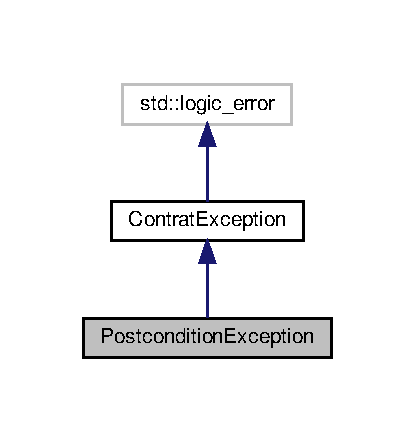
\includegraphics[width=199pt]{classPostconditionException__inherit__graph}
\end{center}
\end{figure}


Collaboration diagram for Postcondition\+Exception\+:\nopagebreak
\begin{figure}[H]
\begin{center}
\leavevmode
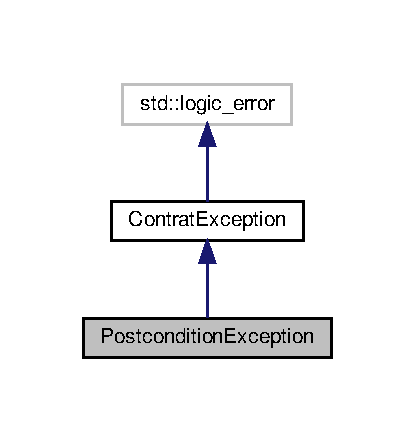
\includegraphics[width=199pt]{classPostconditionException__coll__graph}
\end{center}
\end{figure}
\subsection*{Public Member Functions}
\begin{DoxyCompactItemize}
\item 
\hyperlink{classPostconditionException_acc95ea17c4302b996261b7201d2cf6c4}{Postcondition\+Exception} (std\+::string, unsigned int, std\+::string)
\begin{DoxyCompactList}\small\item\em Constructeur de la classe \hyperlink{classPostconditionException}{Postcondition\+Exception} en initialisant la classe de base \hyperlink{classContratException}{Contrat\+Exception}. La classe représente des erreurs de postcondition dans la théorie du contrat. \end{DoxyCompactList}\end{DoxyCompactItemize}


\subsection{Detailed Description}
Classe pour la gestion des erreurs de postcondition. 

\subsection{Constructor \& Destructor Documentation}
\mbox{\Hypertarget{classPostconditionException_acc95ea17c4302b996261b7201d2cf6c4}\label{classPostconditionException_acc95ea17c4302b996261b7201d2cf6c4}} 
\index{Postcondition\+Exception@{Postcondition\+Exception}!Postcondition\+Exception@{Postcondition\+Exception}}
\index{Postcondition\+Exception@{Postcondition\+Exception}!Postcondition\+Exception@{Postcondition\+Exception}}
\subsubsection{\texorpdfstring{Postcondition\+Exception()}{PostconditionException()}}
{\footnotesize\ttfamily Postcondition\+Exception\+::\+Postcondition\+Exception (\begin{DoxyParamCaption}\item[{std\+::string}]{p\+\_\+fichP,  }\item[{unsigned int}]{p\+\_\+prm\+Ligne,  }\item[{std\+::string}]{p\+\_\+exprP }\end{DoxyParamCaption})}



Constructeur de la classe \hyperlink{classPostconditionException}{Postcondition\+Exception} en initialisant la classe de base \hyperlink{classContratException}{Contrat\+Exception}. La classe représente des erreurs de postcondition dans la théorie du contrat. 


\begin{DoxyParams}{Parameters}
{\em p\+\_\+fichP} & chaîne de caractères représentant le fichier source dans lequel a eu lieu l\textquotesingle{}erreur \\
\hline
{\em p\+\_\+prm\+Ligne} & un entier représentant la ligne où a eu lieu l\textquotesingle{}erreur \\
\hline
{\em p\+\_\+exprP} & Test logique qui a échoué \\
\hline
\end{DoxyParams}


The documentation for this class was generated from the following files\+:\begin{DoxyCompactItemize}
\item 
\hyperlink{ContratException_8h}{Contrat\+Exception.\+h}\item 
\hyperlink{ContratException_8cpp}{Contrat\+Exception.\+cpp}\end{DoxyCompactItemize}

\hypertarget{classPreconditionException}{}\section{Precondition\+Exception Class Reference}
\label{classPreconditionException}\index{Precondition\+Exception@{Precondition\+Exception}}


Classe pour la gestion des erreurs de précondition.  




{\ttfamily \#include $<$Contrat\+Exception.\+h$>$}



Inheritance diagram for Precondition\+Exception\+:\nopagebreak
\begin{figure}[H]
\begin{center}
\leavevmode
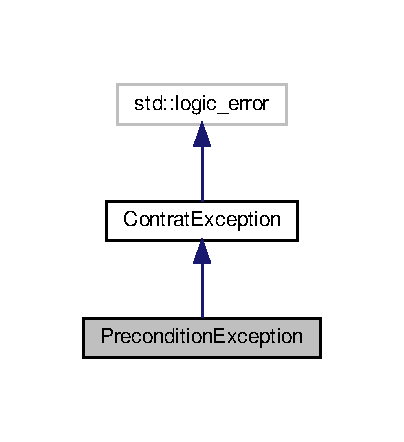
\includegraphics[width=194pt]{classPreconditionException__inherit__graph}
\end{center}
\end{figure}


Collaboration diagram for Precondition\+Exception\+:\nopagebreak
\begin{figure}[H]
\begin{center}
\leavevmode
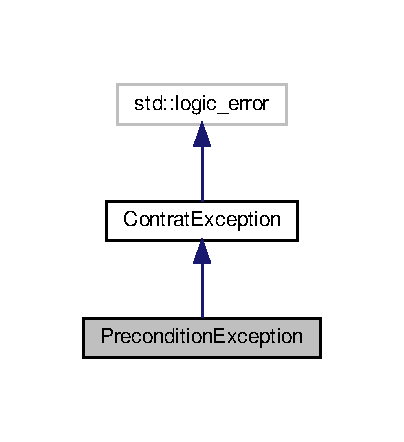
\includegraphics[width=194pt]{classPreconditionException__coll__graph}
\end{center}
\end{figure}
\subsection*{Public Member Functions}
\begin{DoxyCompactItemize}
\item 
\hyperlink{classPreconditionException_a66d4b4c57a0675d487dab85d2c31b08c}{Precondition\+Exception} (std\+::string, unsigned int, std\+::string)
\begin{DoxyCompactList}\small\item\em Constructeur de la classe \hyperlink{classPreconditionException}{Precondition\+Exception} en initialisant la classe de base \hyperlink{classContratException}{Contrat\+Exception}. La classe représente l\textquotesingle{}erreur de précondition dans la théorie du contrat. \end{DoxyCompactList}\end{DoxyCompactItemize}


\subsection{Detailed Description}
Classe pour la gestion des erreurs de précondition. 

\subsection{Constructor \& Destructor Documentation}
\mbox{\Hypertarget{classPreconditionException_a66d4b4c57a0675d487dab85d2c31b08c}\label{classPreconditionException_a66d4b4c57a0675d487dab85d2c31b08c}} 
\index{Precondition\+Exception@{Precondition\+Exception}!Precondition\+Exception@{Precondition\+Exception}}
\index{Precondition\+Exception@{Precondition\+Exception}!Precondition\+Exception@{Precondition\+Exception}}
\subsubsection{\texorpdfstring{Precondition\+Exception()}{PreconditionException()}}
{\footnotesize\ttfamily Precondition\+Exception\+::\+Precondition\+Exception (\begin{DoxyParamCaption}\item[{std\+::string}]{p\+\_\+fichP,  }\item[{unsigned int}]{p\+\_\+prm\+Ligne,  }\item[{std\+::string}]{p\+\_\+exprP }\end{DoxyParamCaption})}



Constructeur de la classe \hyperlink{classPreconditionException}{Precondition\+Exception} en initialisant la classe de base \hyperlink{classContratException}{Contrat\+Exception}. La classe représente l\textquotesingle{}erreur de précondition dans la théorie du contrat. 


\begin{DoxyParams}{Parameters}
{\em p\+\_\+fichP} & chaîne de caractères représentant le fichier source dans lequel a eu lieu l\textquotesingle{}erreur \\
\hline
{\em p\+\_\+prm\+Ligne} & un entier représentant la ligne où a eu lieu l\textquotesingle{}erreur \\
\hline
{\em p\+\_\+exprP} & Test logique qui a échoué \\
\hline
\end{DoxyParams}


The documentation for this class was generated from the following files\+:\begin{DoxyCompactItemize}
\item 
\hyperlink{ContratException_8h}{Contrat\+Exception.\+h}\item 
\hyperlink{ContratException_8cpp}{Contrat\+Exception.\+cpp}\end{DoxyCompactItemize}

\chapter{File Documentation}
\hypertarget{Adresse_8cpp}{}\section{Adresse.\+cpp File Reference}
\label{Adresse_8cpp}\index{Adresse.\+cpp@{Adresse.\+cpp}}


Implantation de la classe Adresse.  


{\ttfamily \#include \char`\"{}Adresse.\+h\char`\"{}}\newline
{\ttfamily \#include $<$string$>$}\newline
{\ttfamily \#include $<$iostream$>$}\newline
{\ttfamily \#include $<$sstream$>$}\newline
Include dependency graph for Adresse.\+cpp\+:\nopagebreak
\begin{figure}[H]
\begin{center}
\leavevmode
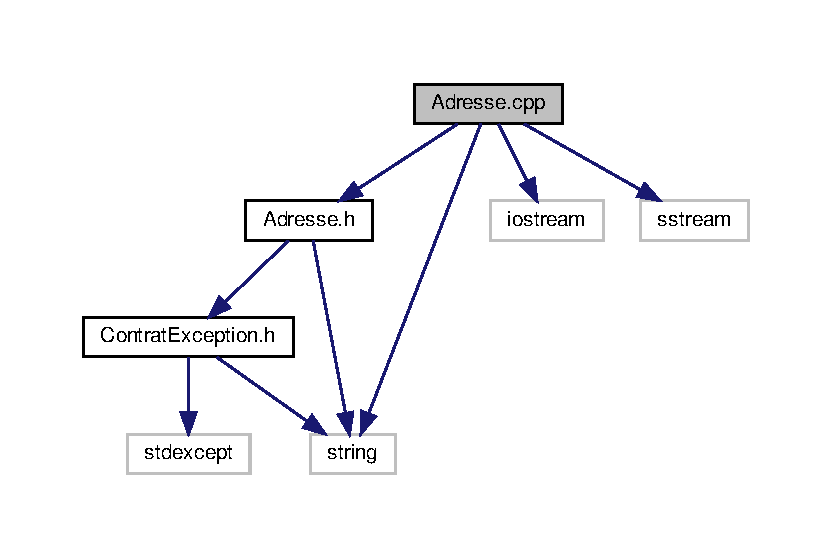
\includegraphics[width=350pt]{Adresse_8cpp__incl}
\end{center}
\end{figure}


\subsection{Detailed Description}
Implantation de la classe Adresse. 

\begin{DoxyAuthor}{Author}
Maxime Imbeau 
\end{DoxyAuthor}
\begin{DoxyVersion}{Version}
0.\+1 
\end{DoxyVersion}
\begin{DoxyDate}{Date}
12/10/2020 
\end{DoxyDate}

\hypertarget{Adresse_8h}{}\section{Adresse.\+h File Reference}
\label{Adresse_8h}\index{Adresse.\+h@{Adresse.\+h}}


Fichier qui contient l\textquotesingle{}interface de la classe Date qui sert au maintien et à la manipulation des adresses.  


{\ttfamily \#include $<$string$>$}\newline
{\ttfamily \#include \char`\"{}Contrat\+Exception.\+h\char`\"{}}\newline
Include dependency graph for Adresse.\+h\+:\nopagebreak
\begin{figure}[H]
\begin{center}
\leavevmode
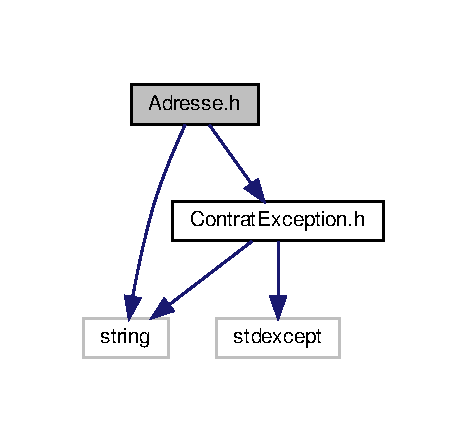
\includegraphics[width=224pt]{Adresse_8h__incl}
\end{center}
\end{figure}
This graph shows which files directly or indirectly include this file\+:\nopagebreak
\begin{figure}[H]
\begin{center}
\leavevmode
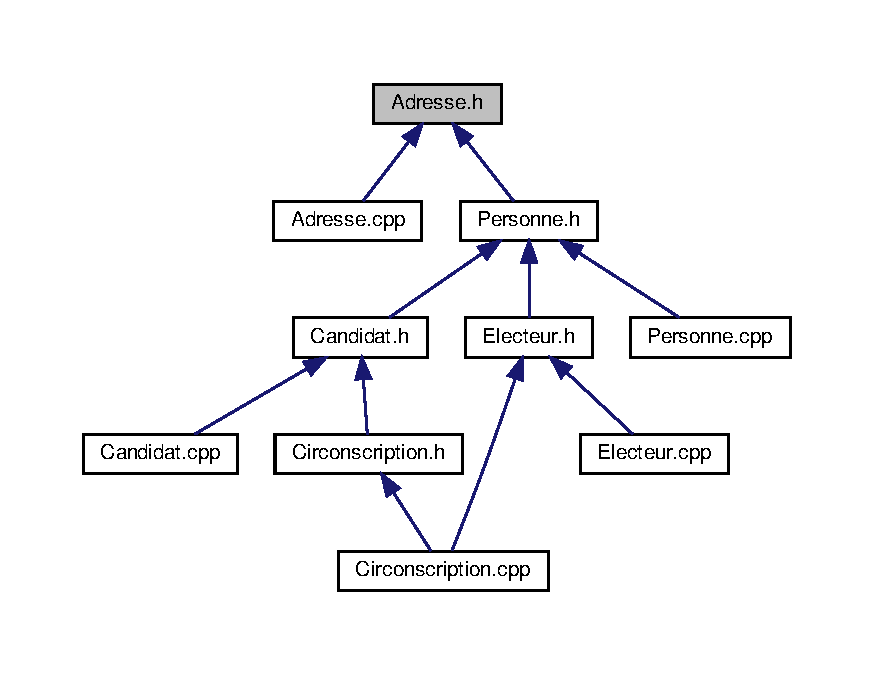
\includegraphics[width=350pt]{Adresse_8h__dep__incl}
\end{center}
\end{figure}
\subsection*{Classes}
\begin{DoxyCompactItemize}
\item 
class \hyperlink{classutil_1_1Adresse}{util\+::\+Adresse}
\begin{DoxyCompactList}\small\item\em Cette classe sert au maintien et à la manipulation des adresses. La classe \hyperlink{classutil_1_1Adresse}{Adresse} permet d\textquotesingle{}implanter des adresses. \end{DoxyCompactList}\end{DoxyCompactItemize}


\subsection{Detailed Description}
Fichier qui contient l\textquotesingle{}interface de la classe Date qui sert au maintien et à la manipulation des adresses. 

\begin{DoxyAuthor}{Author}
Maxime Imbeau 
\end{DoxyAuthor}
\begin{DoxyVersion}{Version}
0.\+1 
\end{DoxyVersion}
\begin{DoxyDate}{Date}
12/10/2020 
\end{DoxyDate}

\hypertarget{Candidat_8cpp}{}\section{Candidat.\+cpp File Reference}
\label{Candidat_8cpp}\index{Candidat.\+cpp@{Candidat.\+cpp}}


Implantation de la classe Candidat.  


{\ttfamily \#include \char`\"{}Candidat.\+h\char`\"{}}\newline
{\ttfamily \#include $<$string$>$}\newline
{\ttfamily \#include $<$iostream$>$}\newline
{\ttfamily \#include $<$sstream$>$}\newline
Include dependency graph for Candidat.\+cpp\+:\nopagebreak
\begin{figure}[H]
\begin{center}
\leavevmode
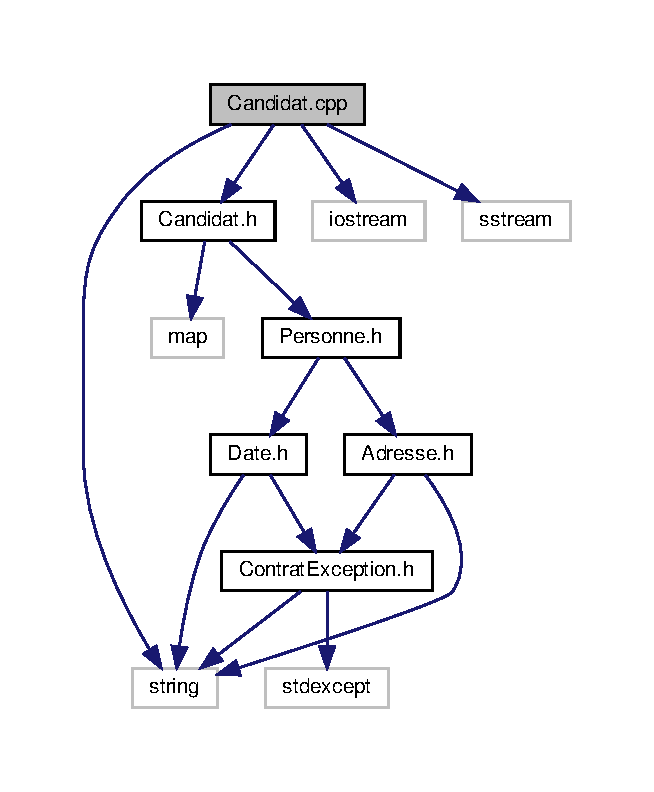
\includegraphics[width=314pt]{Candidat_8cpp__incl}
\end{center}
\end{figure}


\subsection{Detailed Description}
Implantation de la classe Candidat. 

\begin{DoxyAuthor}{Author}
Maxime Imbeau 
\end{DoxyAuthor}
\begin{DoxyVersion}{Version}
0.\+1 
\end{DoxyVersion}
\begin{DoxyDate}{Date}
14/1/2020 
\end{DoxyDate}

\hypertarget{Candidat_8h}{}\section{Candidat.\+h File Reference}
\label{Candidat_8h}\index{Candidat.\+h@{Candidat.\+h}}


Fichier qui contient l\textquotesingle{}interface de la classe Candidat qui sert au maintien et à la manipulation des informations sur un candidat.  


{\ttfamily \#include \char`\"{}Personne.\+h\char`\"{}}\newline
{\ttfamily \#include $<$map$>$}\newline
Include dependency graph for Candidat.\+h\+:\nopagebreak
\begin{figure}[H]
\begin{center}
\leavevmode
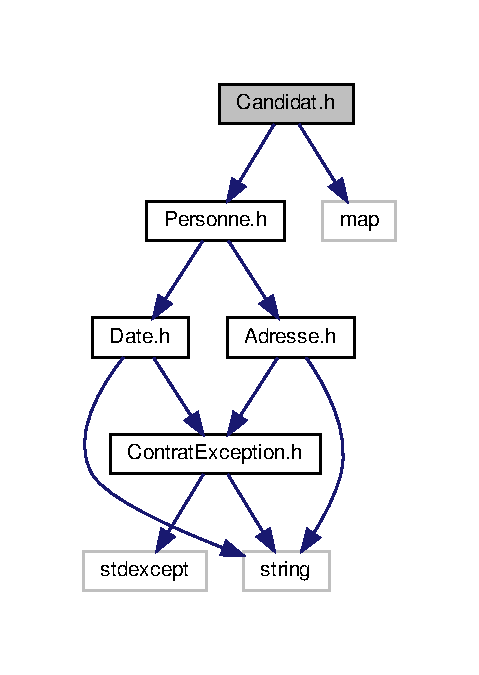
\includegraphics[width=230pt]{Candidat_8h__incl}
\end{center}
\end{figure}
This graph shows which files directly or indirectly include this file\+:\nopagebreak
\begin{figure}[H]
\begin{center}
\leavevmode
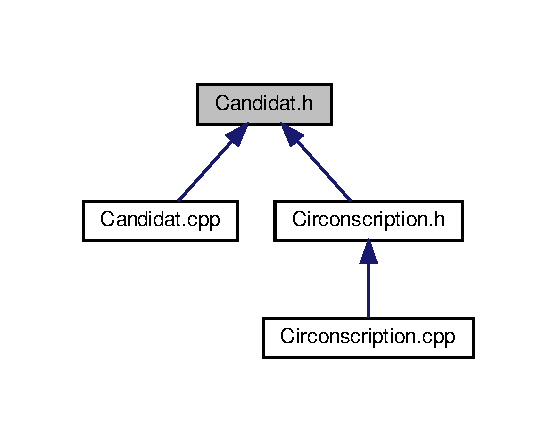
\includegraphics[width=267pt]{Candidat_8h__dep__incl}
\end{center}
\end{figure}
\subsection*{Classes}
\begin{DoxyCompactItemize}
\item 
class \hyperlink{classelections_1_1Candidat}{elections\+::\+Candidat}
\begin{DoxyCompactList}\small\item\em Classe dérivée de la classe \hyperlink{classelections_1_1Personne}{Personne}. \end{DoxyCompactList}\end{DoxyCompactItemize}


\subsection{Detailed Description}
Fichier qui contient l\textquotesingle{}interface de la classe Candidat qui sert au maintien et à la manipulation des informations sur un candidat. 

\begin{DoxyAuthor}{Author}
Maxime Imbeau 
\end{DoxyAuthor}
\begin{DoxyVersion}{Version}
0.\+1 
\end{DoxyVersion}
\begin{DoxyDate}{Date}
14/11/2020 
\end{DoxyDate}

\hypertarget{Circonscription_8cpp}{}\section{Circonscription.\+cpp File Reference}
\label{Circonscription_8cpp}\index{Circonscription.\+cpp@{Circonscription.\+cpp}}


Implantation de la classe Circonscription.  


{\ttfamily \#include \char`\"{}Circonscription.\+h\char`\"{}}\newline
{\ttfamily \#include \char`\"{}Electeur.\+h\char`\"{}}\newline
{\ttfamily \#include $<$string$>$}\newline
{\ttfamily \#include $<$sstream$>$}\newline
{\ttfamily \#include $<$iostream$>$}\newline
Include dependency graph for Circonscription.\+cpp\+:\nopagebreak
\begin{figure}[H]
\begin{center}
\leavevmode
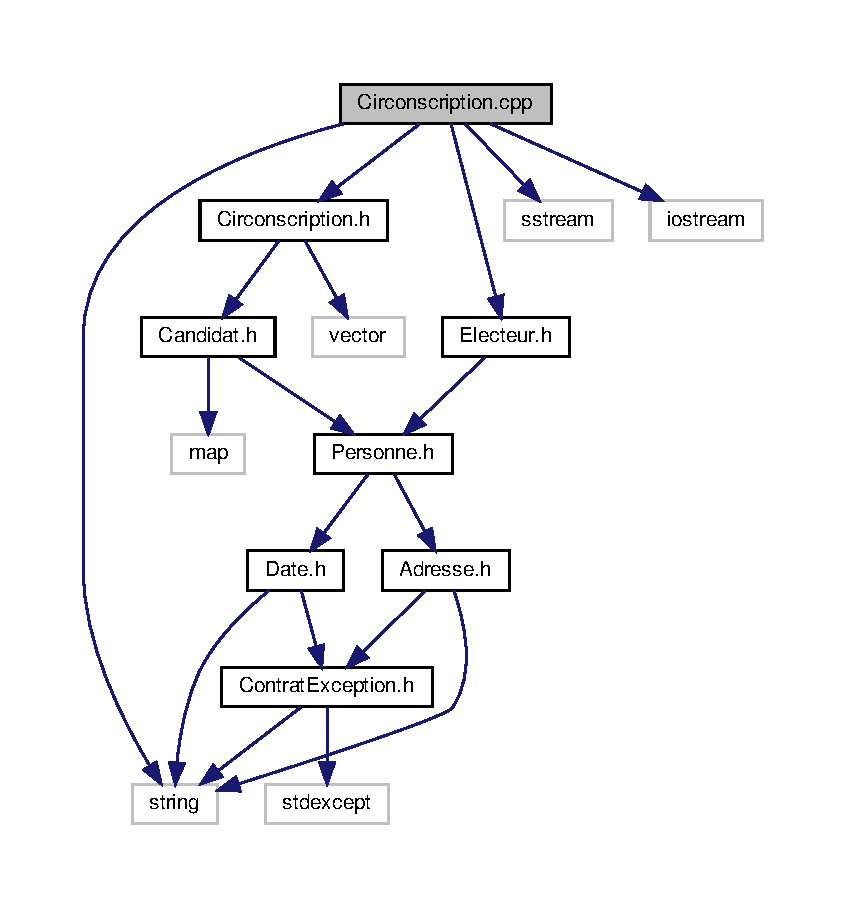
\includegraphics[width=350pt]{Circonscription_8cpp__incl}
\end{center}
\end{figure}


\subsection{Detailed Description}
Implantation de la classe Circonscription. 

\begin{DoxyAuthor}{Author}
Maxime Imbeau 
\end{DoxyAuthor}
\begin{DoxyVersion}{Version}
0.\+1 
\end{DoxyVersion}
\begin{DoxyDate}{Date}
14/1/2020 
\end{DoxyDate}

\hypertarget{Circonscription_8h}{}\section{Circonscription.\+h File Reference}
\label{Circonscription_8h}\index{Circonscription.\+h@{Circonscription.\+h}}


Fichier qui contient l\textquotesingle{}interface de la classe Circonscription qui permet de faire la gestion des listes électorales.  


{\ttfamily \#include \char`\"{}Candidat.\+h\char`\"{}}\newline
{\ttfamily \#include $<$vector$>$}\newline
Include dependency graph for Circonscription.\+h\+:\nopagebreak
\begin{figure}[H]
\begin{center}
\leavevmode
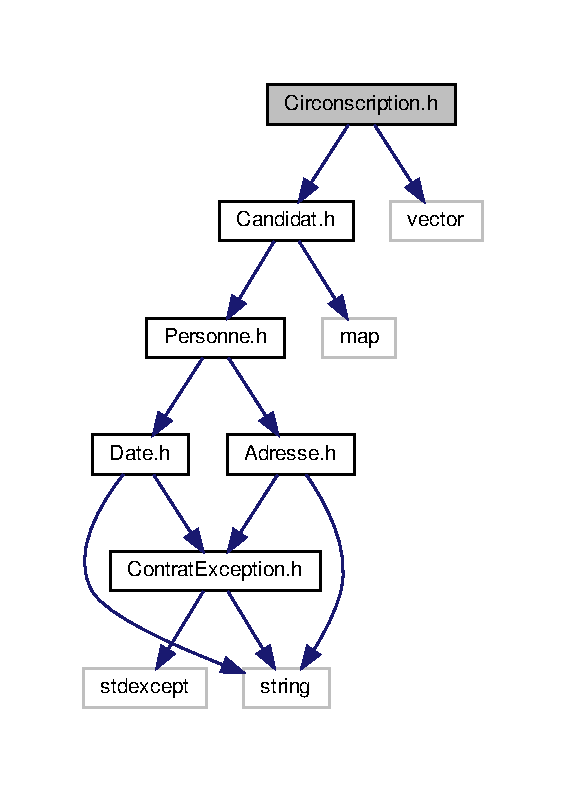
\includegraphics[width=271pt]{Circonscription_8h__incl}
\end{center}
\end{figure}
This graph shows which files directly or indirectly include this file\+:\nopagebreak
\begin{figure}[H]
\begin{center}
\leavevmode
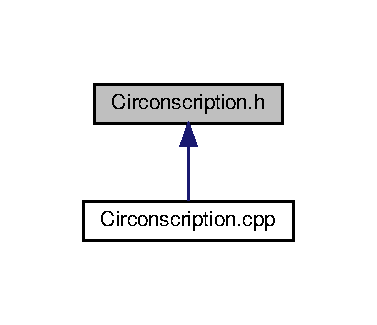
\includegraphics[width=181pt]{Circonscription_8h__dep__incl}
\end{center}
\end{figure}
\subsection*{Classes}
\begin{DoxyCompactItemize}
\item 
class \hyperlink{classelections_1_1Circonscription}{elections\+::\+Circonscription}
\begin{DoxyCompactList}\small\item\em La classe \hyperlink{classelections_1_1Circonscription}{Circonscription} permet de faire la gestion des listes électorales. \end{DoxyCompactList}\end{DoxyCompactItemize}


\subsection{Detailed Description}
Fichier qui contient l\textquotesingle{}interface de la classe Circonscription qui permet de faire la gestion des listes électorales. 

\begin{DoxyAuthor}{Author}
Maxime Imbeau 
\end{DoxyAuthor}
\begin{DoxyVersion}{Version}
0.\+1 
\end{DoxyVersion}
\begin{DoxyDate}{Date}
14/11/2020 
\end{DoxyDate}

\hypertarget{ContratException_8cpp}{}\section{Contrat\+Exception.\+cpp File Reference}
\label{ContratException_8cpp}\index{Contrat\+Exception.\+cpp@{Contrat\+Exception.\+cpp}}


Implantation de la classe \hyperlink{classContratException}{Contrat\+Exception} et de ses héritiers.  


{\ttfamily \#include \char`\"{}Contrat\+Exception.\+h\char`\"{}}\newline
{\ttfamily \#include $<$sstream$>$}\newline
Include dependency graph for Contrat\+Exception.\+cpp\+:\nopagebreak
\begin{figure}[H]
\begin{center}
\leavevmode
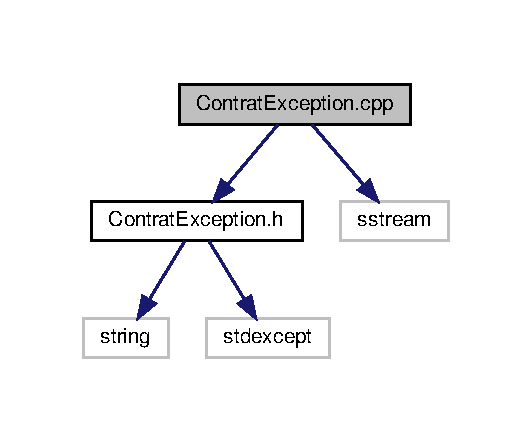
\includegraphics[width=255pt]{ContratException_8cpp__incl}
\end{center}
\end{figure}


\subsection{Detailed Description}
Implantation de la classe \hyperlink{classContratException}{Contrat\+Exception} et de ses héritiers. 

\begin{DoxyAuthor}{Author}
administrateur 
\end{DoxyAuthor}

\hypertarget{ContratException_8h}{}\section{Contrat\+Exception.\+h File Reference}
\label{ContratException_8h}\index{Contrat\+Exception.\+h@{Contrat\+Exception.\+h}}


Fichier contenant la déclaration de la classe \hyperlink{classContratException}{Contrat\+Exception} et de ses héritiers.  


{\ttfamily \#include $<$string$>$}\newline
{\ttfamily \#include $<$stdexcept$>$}\newline
Include dependency graph for Contrat\+Exception.\+h\+:\nopagebreak
\begin{figure}[H]
\begin{center}
\leavevmode
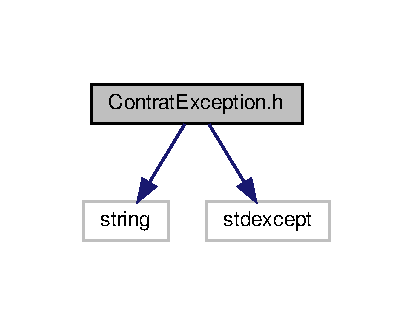
\includegraphics[width=198pt]{ContratException_8h__incl}
\end{center}
\end{figure}
This graph shows which files directly or indirectly include this file\+:\nopagebreak
\begin{figure}[H]
\begin{center}
\leavevmode
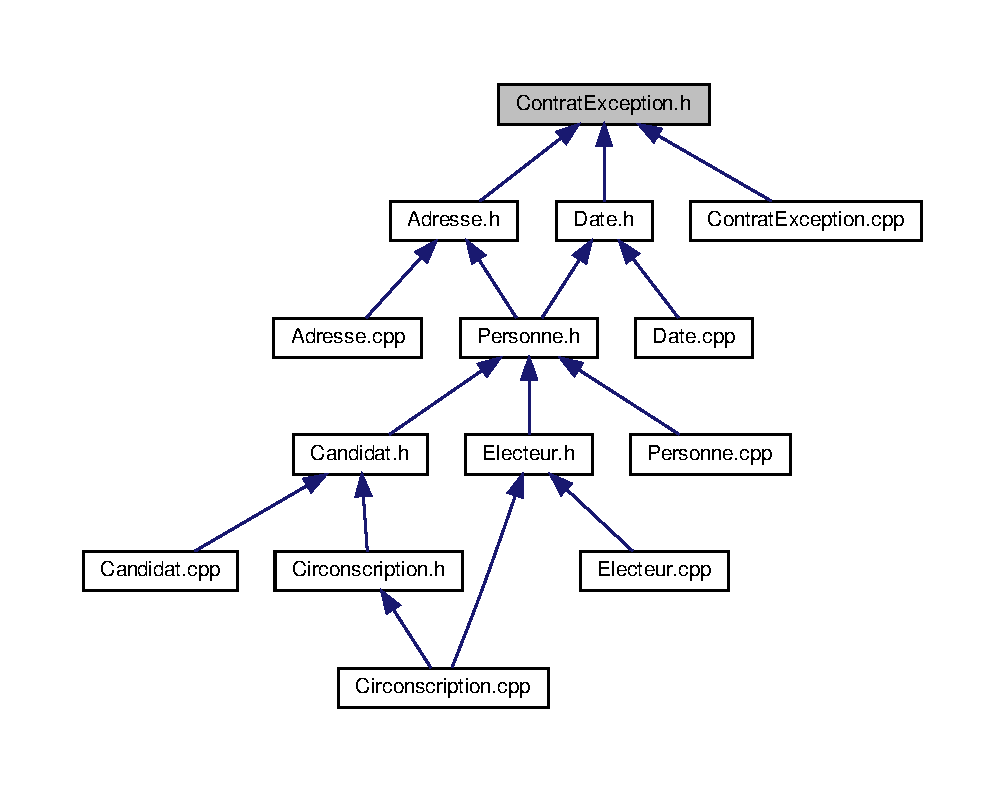
\includegraphics[width=350pt]{ContratException_8h__dep__incl}
\end{center}
\end{figure}
\subsection*{Classes}
\begin{DoxyCompactItemize}
\item 
class \hyperlink{classContratException}{Contrat\+Exception}
\begin{DoxyCompactList}\small\item\em Classe de base des exceptions de contrat. \end{DoxyCompactList}\item 
class \hyperlink{classAssertionException}{Assertion\+Exception}
\begin{DoxyCompactList}\small\item\em Classe pour la gestion des erreurs d\textquotesingle{}assertion. \end{DoxyCompactList}\item 
class \hyperlink{classPreconditionException}{Precondition\+Exception}
\begin{DoxyCompactList}\small\item\em Classe pour la gestion des erreurs de précondition. \end{DoxyCompactList}\item 
class \hyperlink{classPostconditionException}{Postcondition\+Exception}
\begin{DoxyCompactList}\small\item\em Classe pour la gestion des erreurs de postcondition. \end{DoxyCompactList}\item 
class \hyperlink{classInvariantException}{Invariant\+Exception}
\begin{DoxyCompactList}\small\item\em Classe pour la gestion des erreurs d\textquotesingle{}invariant. \end{DoxyCompactList}\end{DoxyCompactItemize}
\subsection*{Macros}
\begin{DoxyCompactItemize}
\item 
\mbox{\Hypertarget{ContratException_8h_a52dddc2c198c58b53b201c313934e40c}\label{ContratException_8h_a52dddc2c198c58b53b201c313934e40c}} 
\#define {\bfseries I\+N\+V\+A\+R\+I\+A\+N\+TS}()~verifie\+Invariant()
\item 
\mbox{\Hypertarget{ContratException_8h_abe6e3e0ff48f8595570e6485b506a8c4}\label{ContratException_8h_abe6e3e0ff48f8595570e6485b506a8c4}} 
\#define {\bfseries A\+S\+S\+E\+R\+T\+I\+ON}(f)~if (!(f)) throw \hyperlink{classAssertionException}{Assertion\+Exception}(\+\_\+\+\_\+\+F\+I\+L\+E\+\_\+\+\_\+,\+\_\+\+\_\+\+L\+I\+N\+E\+\_\+\+\_\+, \#f);
\item 
\mbox{\Hypertarget{ContratException_8h_acb3361bd87fc697a57b7286a9998c106}\label{ContratException_8h_acb3361bd87fc697a57b7286a9998c106}} 
\#define {\bfseries P\+R\+E\+C\+O\+N\+D\+I\+T\+I\+ON}(f)~if (!(f)) throw \hyperlink{classPreconditionException}{Precondition\+Exception}(\+\_\+\+\_\+\+F\+I\+L\+E\+\_\+\+\_\+, \+\_\+\+\_\+\+L\+I\+N\+E\+\_\+\+\_\+, \#f);
\item 
\mbox{\Hypertarget{ContratException_8h_a438b75c0c77a1ce8d1e914f9f04ea548}\label{ContratException_8h_a438b75c0c77a1ce8d1e914f9f04ea548}} 
\#define {\bfseries P\+O\+S\+T\+C\+O\+N\+D\+I\+T\+I\+ON}(f)~if (!(f)) throw \hyperlink{classPostconditionException}{Postcondition\+Exception}(\+\_\+\+\_\+\+F\+I\+L\+E\+\_\+\+\_\+, \+\_\+\+\_\+\+L\+I\+N\+E\+\_\+\+\_\+, \#f);
\item 
\mbox{\Hypertarget{ContratException_8h_a08f80155f47e05681c2b9bb9c5f6fffe}\label{ContratException_8h_a08f80155f47e05681c2b9bb9c5f6fffe}} 
\#define {\bfseries I\+N\+V\+A\+R\+I\+A\+NT}(f)~if (!(f)) throw \hyperlink{classInvariantException}{Invariant\+Exception}(\+\_\+\+\_\+\+F\+I\+L\+E\+\_\+\+\_\+,\+\_\+\+\_\+\+L\+I\+N\+E\+\_\+\+\_\+, \#f);
\end{DoxyCompactItemize}


\subsection{Detailed Description}
Fichier contenant la déclaration de la classe \hyperlink{classContratException}{Contrat\+Exception} et de ses héritiers. 

\begin{DoxyAuthor}{Author}
administrateur 
\end{DoxyAuthor}

\hypertarget{Date_8cpp}{}\section{Date.\+cpp File Reference}
\label{Date_8cpp}\index{Date.\+cpp@{Date.\+cpp}}


Implantation de la classe Date révision \+: normes 12-\/2013 balises Doxygen révision des commentaires de spécification d\textquotesingle{}en-\/tête des méthodes.  


{\ttfamily \#include \char`\"{}Date.\+h\char`\"{}}\newline
{\ttfamily \#include $<$sstream$>$}\newline
{\ttfamily \#include $<$ctime$>$}\newline
{\ttfamily \#include $<$iostream$>$}\newline
Include dependency graph for Date.\+cpp\+:\nopagebreak
\begin{figure}[H]
\begin{center}
\leavevmode
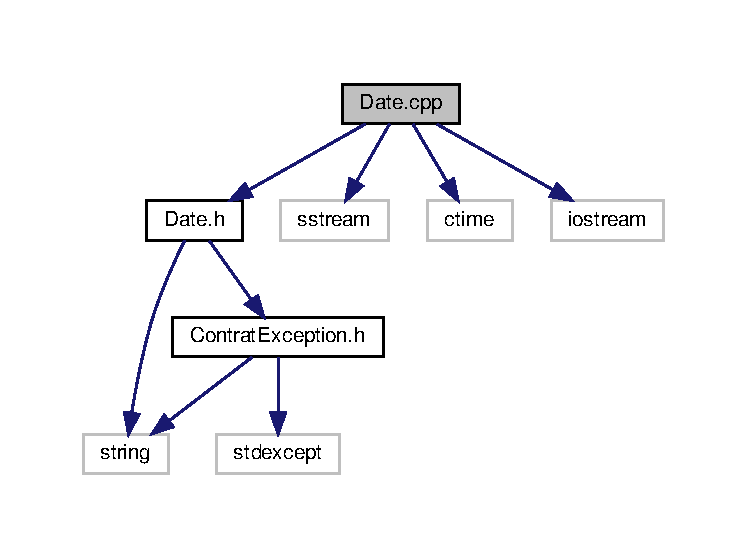
\includegraphics[width=350pt]{Date_8cpp__incl}
\end{center}
\end{figure}


\subsection{Detailed Description}
Implantation de la classe Date révision \+: normes 12-\/2013 balises Doxygen révision des commentaires de spécification d\textquotesingle{}en-\/tête des méthodes. 

\begin{DoxyAuthor}{Author}
Yves Roy Version initiale, T\+HE 
\end{DoxyAuthor}
\begin{DoxyDate}{Date}
28 octobre 2016 
\end{DoxyDate}
\begin{DoxyVersion}{Version}
2.\+4 
\end{DoxyVersion}

\hypertarget{Date_8h}{}\section{Date.\+h File Reference}
\label{Date_8h}\index{Date.\+h@{Date.\+h}}


Fichier qui contient l\textquotesingle{}interface de la classe Date qui sert au maintien et à la manipulation des dates.  


{\ttfamily \#include \char`\"{}Contrat\+Exception.\+h\char`\"{}}\newline
{\ttfamily \#include $<$string$>$}\newline
Include dependency graph for Date.\+h\+:\nopagebreak
\begin{figure}[H]
\begin{center}
\leavevmode
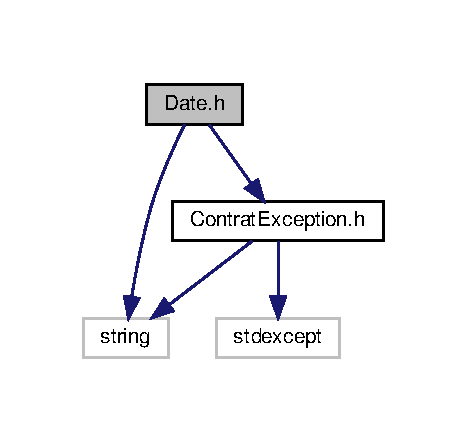
\includegraphics[width=224pt]{Date_8h__incl}
\end{center}
\end{figure}
This graph shows which files directly or indirectly include this file\+:\nopagebreak
\begin{figure}[H]
\begin{center}
\leavevmode
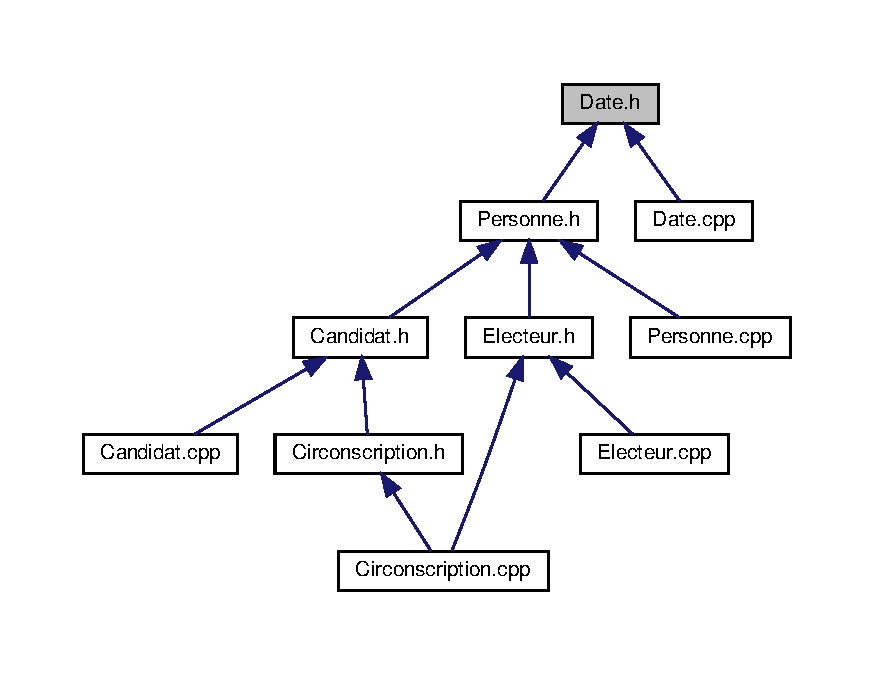
\includegraphics[width=350pt]{Date_8h__dep__incl}
\end{center}
\end{figure}
\subsection*{Classes}
\begin{DoxyCompactItemize}
\item 
class \hyperlink{classutil_1_1Date}{util\+::\+Date}
\begin{DoxyCompactList}\small\item\em Cette classe sert au maintien et à la manipulation des dates. \end{DoxyCompactList}\end{DoxyCompactItemize}


\subsection{Detailed Description}
Fichier qui contient l\textquotesingle{}interface de la classe Date qui sert au maintien et à la manipulation des dates. 

\begin{DoxyAuthor}{Author}
Yves Roy Version initiale, T\+HE 
\end{DoxyAuthor}
\begin{DoxyDate}{Date}
28 octobre 2016 
\end{DoxyDate}
\begin{DoxyVersion}{Version}
2.\+2 
\end{DoxyVersion}

\hypertarget{Electeur_8cpp}{}\section{Electeur.\+cpp File Reference}
\label{Electeur_8cpp}\index{Electeur.\+cpp@{Electeur.\+cpp}}


Implantation de la classe Electeur.  


{\ttfamily \#include \char`\"{}Electeur.\+h\char`\"{}}\newline
{\ttfamily \#include $<$string$>$}\newline
{\ttfamily \#include $<$iostream$>$}\newline
{\ttfamily \#include $<$sstream$>$}\newline
Include dependency graph for Electeur.\+cpp\+:\nopagebreak
\begin{figure}[H]
\begin{center}
\leavevmode
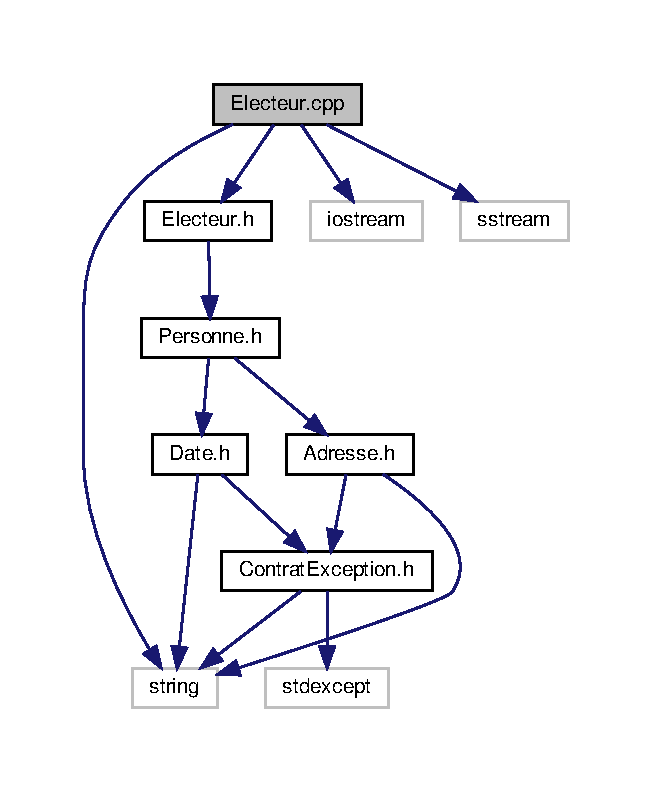
\includegraphics[width=313pt]{Electeur_8cpp__incl}
\end{center}
\end{figure}


\subsection{Detailed Description}
Implantation de la classe Electeur. 

\begin{DoxyAuthor}{Author}
Maxime Imbeau 
\end{DoxyAuthor}
\begin{DoxyVersion}{Version}
0.\+1 
\end{DoxyVersion}
\begin{DoxyDate}{Date}
14/1/2020 
\end{DoxyDate}

\hypertarget{Electeur_8h}{}\section{Electeur.\+h File Reference}
\label{Electeur_8h}\index{Electeur.\+h@{Electeur.\+h}}


Fichier qui contient l\textquotesingle{}interface de la classe Electeur qui sert au maintien et à la manipulation des informations sur un electeur.  


{\ttfamily \#include \char`\"{}Personne.\+h\char`\"{}}\newline
Include dependency graph for Electeur.\+h\+:\nopagebreak
\begin{figure}[H]
\begin{center}
\leavevmode
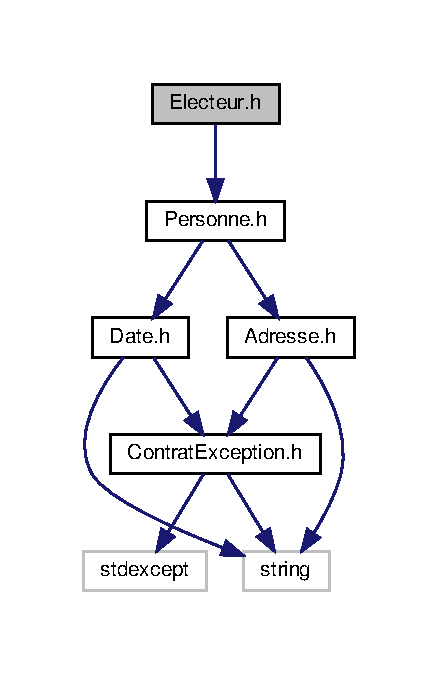
\includegraphics[width=210pt]{Electeur_8h__incl}
\end{center}
\end{figure}
This graph shows which files directly or indirectly include this file\+:\nopagebreak
\begin{figure}[H]
\begin{center}
\leavevmode
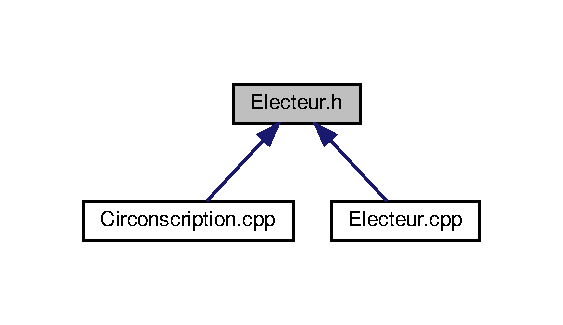
\includegraphics[width=270pt]{Electeur_8h__dep__incl}
\end{center}
\end{figure}
\subsection*{Classes}
\begin{DoxyCompactItemize}
\item 
class \hyperlink{classelections_1_1Electeur}{elections\+::\+Electeur}
\begin{DoxyCompactList}\small\item\em Classe dérivée de la classe \hyperlink{classelections_1_1Personne}{Personne}. \end{DoxyCompactList}\end{DoxyCompactItemize}


\subsection{Detailed Description}
Fichier qui contient l\textquotesingle{}interface de la classe Electeur qui sert au maintien et à la manipulation des informations sur un electeur. 

\begin{DoxyAuthor}{Author}
Maxime Imbeau 
\end{DoxyAuthor}
\begin{DoxyVersion}{Version}
0.\+1 
\end{DoxyVersion}
\begin{DoxyDate}{Date}
14/11/2020 
\end{DoxyDate}

\hypertarget{Personne_8cpp}{}\section{Personne.\+cpp File Reference}
\label{Personne_8cpp}\index{Personne.\+cpp@{Personne.\+cpp}}


Implantation de la classe Personne.  


{\ttfamily \#include \char`\"{}Personne.\+h\char`\"{}}\newline
{\ttfamily \#include \char`\"{}validation\+Format.\+h\char`\"{}}\newline
{\ttfamily \#include $<$string$>$}\newline
{\ttfamily \#include $<$iostream$>$}\newline
{\ttfamily \#include $<$sstream$>$}\newline
Include dependency graph for Personne.\+cpp\+:\nopagebreak
\begin{figure}[H]
\begin{center}
\leavevmode
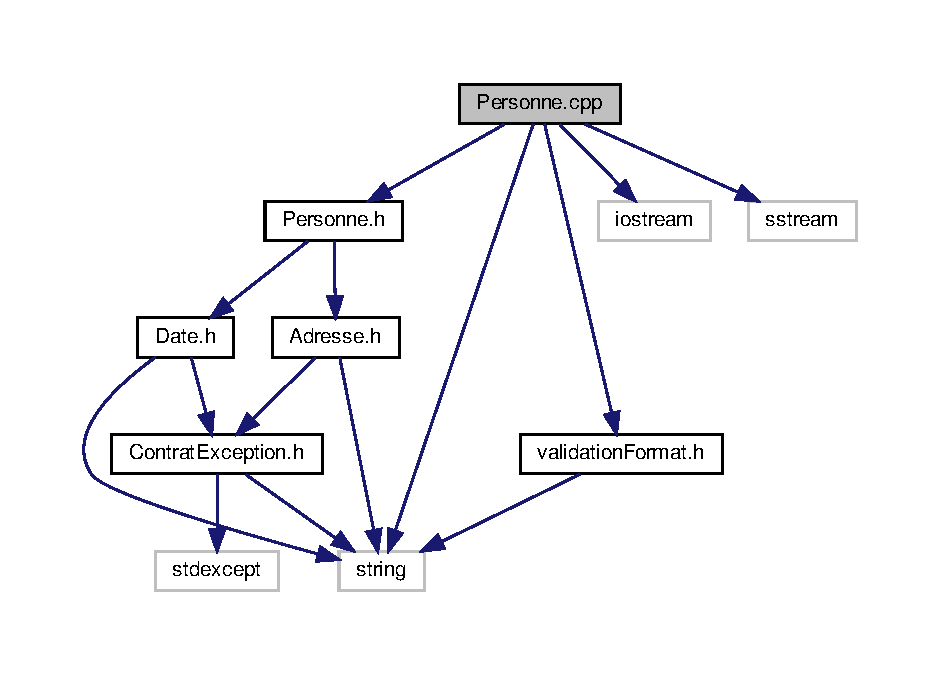
\includegraphics[width=350pt]{Personne_8cpp__incl}
\end{center}
\end{figure}


\subsection{Detailed Description}
Implantation de la classe Personne. 

\begin{DoxyAuthor}{Author}
Maxime Imbeau 
\end{DoxyAuthor}
\begin{DoxyVersion}{Version}
0.\+1 
\end{DoxyVersion}
\begin{DoxyDate}{Date}
12/10/2020 
\end{DoxyDate}

\hypertarget{Personne_8h}{}\section{Personne.\+h File Reference}
\label{Personne_8h}\index{Personne.\+h@{Personne.\+h}}


Fichier qui contient l\textquotesingle{}interface de la classe Personne qui sert au maintien et à la manipulation des informations sur une personne.  


{\ttfamily \#include \char`\"{}Adresse.\+h\char`\"{}}\newline
{\ttfamily \#include \char`\"{}Date.\+h\char`\"{}}\newline
Include dependency graph for Personne.\+h\+:\nopagebreak
\begin{figure}[H]
\begin{center}
\leavevmode
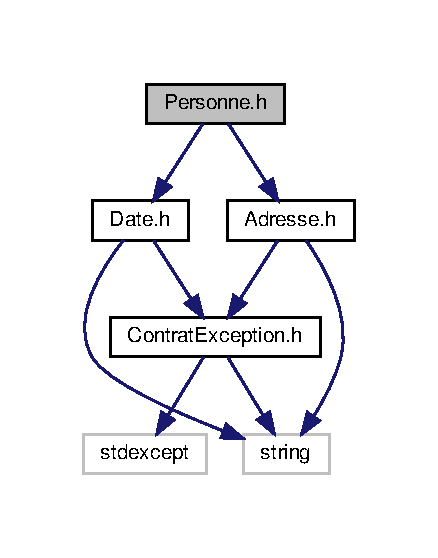
\includegraphics[width=210pt]{Personne_8h__incl}
\end{center}
\end{figure}
This graph shows which files directly or indirectly include this file\+:\nopagebreak
\begin{figure}[H]
\begin{center}
\leavevmode
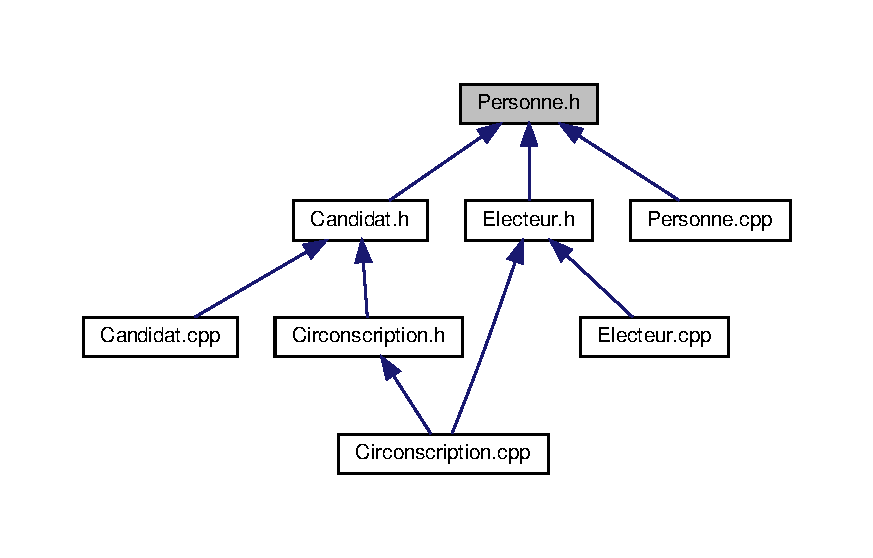
\includegraphics[width=350pt]{Personne_8h__dep__incl}
\end{center}
\end{figure}
\subsection*{Classes}
\begin{DoxyCompactItemize}
\item 
class \hyperlink{classelections_1_1Personne}{elections\+::\+Personne}
\begin{DoxyCompactList}\small\item\em Cette classe sert au maintien et à la manipulation des informations sur une personne. La classe \hyperlink{classelections_1_1Personne}{Personne} permet d\textquotesingle{}implanter des personnes. \end{DoxyCompactList}\end{DoxyCompactItemize}


\subsection{Detailed Description}
Fichier qui contient l\textquotesingle{}interface de la classe Personne qui sert au maintien et à la manipulation des informations sur une personne. 

\begin{DoxyAuthor}{Author}
Maxime Imbeau 
\end{DoxyAuthor}
\begin{DoxyVersion}{Version}
0.\+1 
\end{DoxyVersion}
\begin{DoxyDate}{Date}
12/10/2020 
\end{DoxyDate}

\hypertarget{validationFormat_8cpp}{}\section{validation\+Format.\+cpp File Reference}
\label{validationFormat_8cpp}\index{validation\+Format.\+cpp@{validation\+Format.\+cpp}}


Fonctions qui permettent de valider un N\+AS et de valider le format d\textquotesingle{}un fichier.  


{\ttfamily \#include \char`\"{}validation\+Format.\+h\char`\"{}}\newline
{\ttfamily \#include $<$iostream$>$}\newline
{\ttfamily \#include $<$string$>$}\newline
{\ttfamily \#include $<$sstream$>$}\newline
{\ttfamily \#include $<$cctype$>$}\newline
{\ttfamily \#include $<$stdlib.\+h$>$}\newline
{\ttfamily \#include $<$fstream$>$}\newline
Include dependency graph for validation\+Format.\+cpp\+:\nopagebreak
\begin{figure}[H]
\begin{center}
\leavevmode
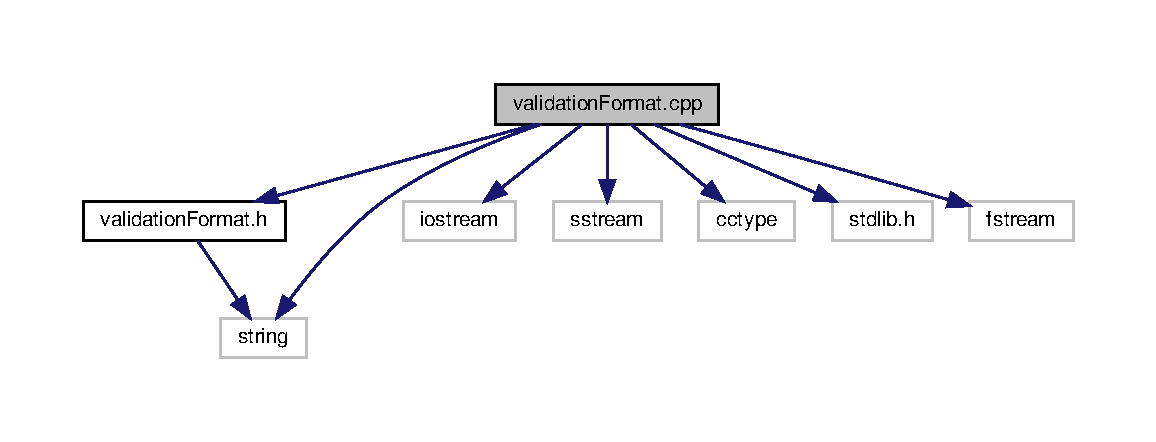
\includegraphics[width=350pt]{validationFormat_8cpp__incl}
\end{center}
\end{figure}
\subsection*{Functions}
\begin{DoxyCompactItemize}
\item 
bool \hyperlink{validationFormat_8cpp_a0ce75a9c4d1aa7f4656d49ef5d206bf3}{util\+::valider\+Nas} (const string \&p\+\_\+nas)
\begin{DoxyCompactList}\small\item\em Vérifie la validité d\textquotesingle{}un N\+AS. \end{DoxyCompactList}\item 
bool \hyperlink{validationFormat_8cpp_a694c704b69cfc694c8b7ba5fd4b34772}{util\+::valider\+Format\+Fichier} (istream \&p\+\_\+is)
\begin{DoxyCompactList}\small\item\em Vérifie la validité du format d\textquotesingle{}un fichier. \end{DoxyCompactList}\end{DoxyCompactItemize}


\subsection{Detailed Description}
Fonctions qui permettent de valider un N\+AS et de valider le format d\textquotesingle{}un fichier. 

\begin{DoxyAuthor}{Author}
Maxime Imbeau 
\end{DoxyAuthor}
\begin{DoxyVersion}{Version}
0.\+1 
\end{DoxyVersion}
\begin{DoxyDate}{Date}
12/10/2020 
\end{DoxyDate}


\subsection{Function Documentation}
\mbox{\Hypertarget{validationFormat_8cpp_file_a694c704b69cfc694c8b7ba5fd4b34772}\label{validationFormat_8cpp_file_a694c704b69cfc694c8b7ba5fd4b34772}} 
\index{validation\+Format.\+cpp@{validation\+Format.\+cpp}!valider\+Format\+Fichier@{valider\+Format\+Fichier}}
\index{valider\+Format\+Fichier@{valider\+Format\+Fichier}!validation\+Format.\+cpp@{validation\+Format.\+cpp}}
\subsubsection{\texorpdfstring{valider\+Format\+Fichier()}{validerFormatFichier()}}
{\footnotesize\ttfamily bool util\+::valider\+Format\+Fichier (\begin{DoxyParamCaption}\item[{istream \&}]{p\+\_\+is }\end{DoxyParamCaption})}



Vérifie la validité du format d\textquotesingle{}un fichier. 


\begin{DoxyParams}[1]{Parameters}
\mbox{\tt in}  & {\em p\+\_\+is} & qui represente un fichier.\+txt \\
\hline
\end{DoxyParams}
\begin{DoxyReturn}{Returns}
un booléen indiquant si le format du fichier est valide ou non 
\end{DoxyReturn}
\mbox{\Hypertarget{validationFormat_8cpp_file_a0ce75a9c4d1aa7f4656d49ef5d206bf3}\label{validationFormat_8cpp_file_a0ce75a9c4d1aa7f4656d49ef5d206bf3}} 
\index{validation\+Format.\+cpp@{validation\+Format.\+cpp}!valider\+Nas@{valider\+Nas}}
\index{valider\+Nas@{valider\+Nas}!validation\+Format.\+cpp@{validation\+Format.\+cpp}}
\subsubsection{\texorpdfstring{valider\+Nas()}{validerNas()}}
{\footnotesize\ttfamily bool util\+::valider\+Nas (\begin{DoxyParamCaption}\item[{const string \&}]{p\+\_\+nas }\end{DoxyParamCaption})}



Vérifie la validité d\textquotesingle{}un N\+AS. 


\begin{DoxyParams}[1]{Parameters}
\mbox{\tt in}  & {\em p\+\_\+nas} & qui represente un numero d\textquotesingle{}assurance social (N\+AS) \\
\hline
\end{DoxyParams}
\begin{DoxyReturn}{Returns}
un booléen indiquant si le N\+AS est valide ou non 
\end{DoxyReturn}

\hypertarget{validationFormat_8h}{}\section{validation\+Format.\+h File Reference}
\label{validationFormat_8h}\index{validation\+Format.\+h@{validation\+Format.\+h}}


Fichier qui contient l\textquotesingle{}interface du fichier de validation d\textquotesingle{}une N\+AS et du format d\textquotesingle{}un fichier.  


{\ttfamily \#include $<$string$>$}\newline
Include dependency graph for validation\+Format.\+h\+:\nopagebreak
\begin{figure}[H]
\begin{center}
\leavevmode
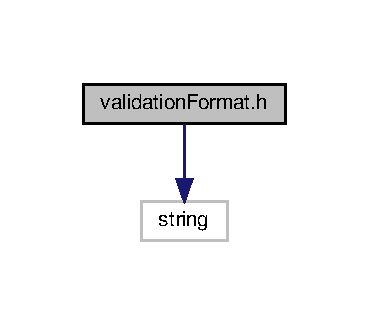
\includegraphics[width=177pt]{validationFormat_8h__incl}
\end{center}
\end{figure}
This graph shows which files directly or indirectly include this file\+:\nopagebreak
\begin{figure}[H]
\begin{center}
\leavevmode
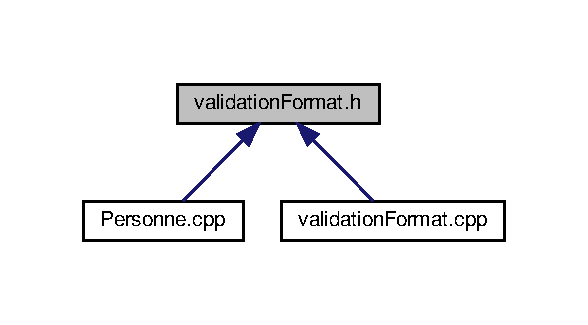
\includegraphics[width=282pt]{validationFormat_8h__dep__incl}
\end{center}
\end{figure}
\subsection*{Functions}
\begin{DoxyCompactItemize}
\item 
\mbox{\Hypertarget{validationFormat_8h_a74e08c8e001753f7dea66351619ca70d}\label{validationFormat_8h_a74e08c8e001753f7dea66351619ca70d}} 
bool {\bfseries util\+::valider\+Nas} (const std\+::string \&p\+\_\+nas)
\item 
\mbox{\Hypertarget{validationFormat_8h_a29d923130070894f0812166f22850c5a}\label{validationFormat_8h_a29d923130070894f0812166f22850c5a}} 
bool {\bfseries util\+::valider\+Format\+Fichier} (std\+::istream \&p\+\_\+is)
\end{DoxyCompactItemize}
\subsection*{Variables}
\begin{DoxyCompactItemize}
\item 
\mbox{\Hypertarget{validationFormat_8h_a87c54fe5fd2e3bcd69a59c6643d0511c}\label{validationFormat_8h_a87c54fe5fd2e3bcd69a59c6643d0511c}} 
const int {\bfseries util\+::\+M\+AX} = 11
\item 
\mbox{\Hypertarget{validationFormat_8h_a19d165dc4e66c9347b76a7b68a836c9f}\label{validationFormat_8h_a19d165dc4e66c9347b76a7b68a836c9f}} 
const int {\bfseries util\+::nb\+\_\+parti} = 5
\end{DoxyCompactItemize}


\subsection{Detailed Description}
Fichier qui contient l\textquotesingle{}interface du fichier de validation d\textquotesingle{}une N\+AS et du format d\textquotesingle{}un fichier. 

\begin{DoxyAuthor}{Author}
Maxime Imbeau 
\end{DoxyAuthor}
\begin{DoxyVersion}{Version}
0.\+1 
\end{DoxyVersion}
\begin{DoxyDate}{Date}
12/10/2020 
\end{DoxyDate}

%--- End generated contents ---

% Index
\backmatter
\newpage
\phantomsection
\clearemptydoublepage
\addcontentsline{toc}{chapter}{Index}
\printindex

\end{document}
